\chapter{Architectural Design}

\section{Overview}
The architecture of the platform is divided into three layers. The figure below represents a high-level description of the components that make up the BBP application. 

\begin{figure}[H]
    \centering
    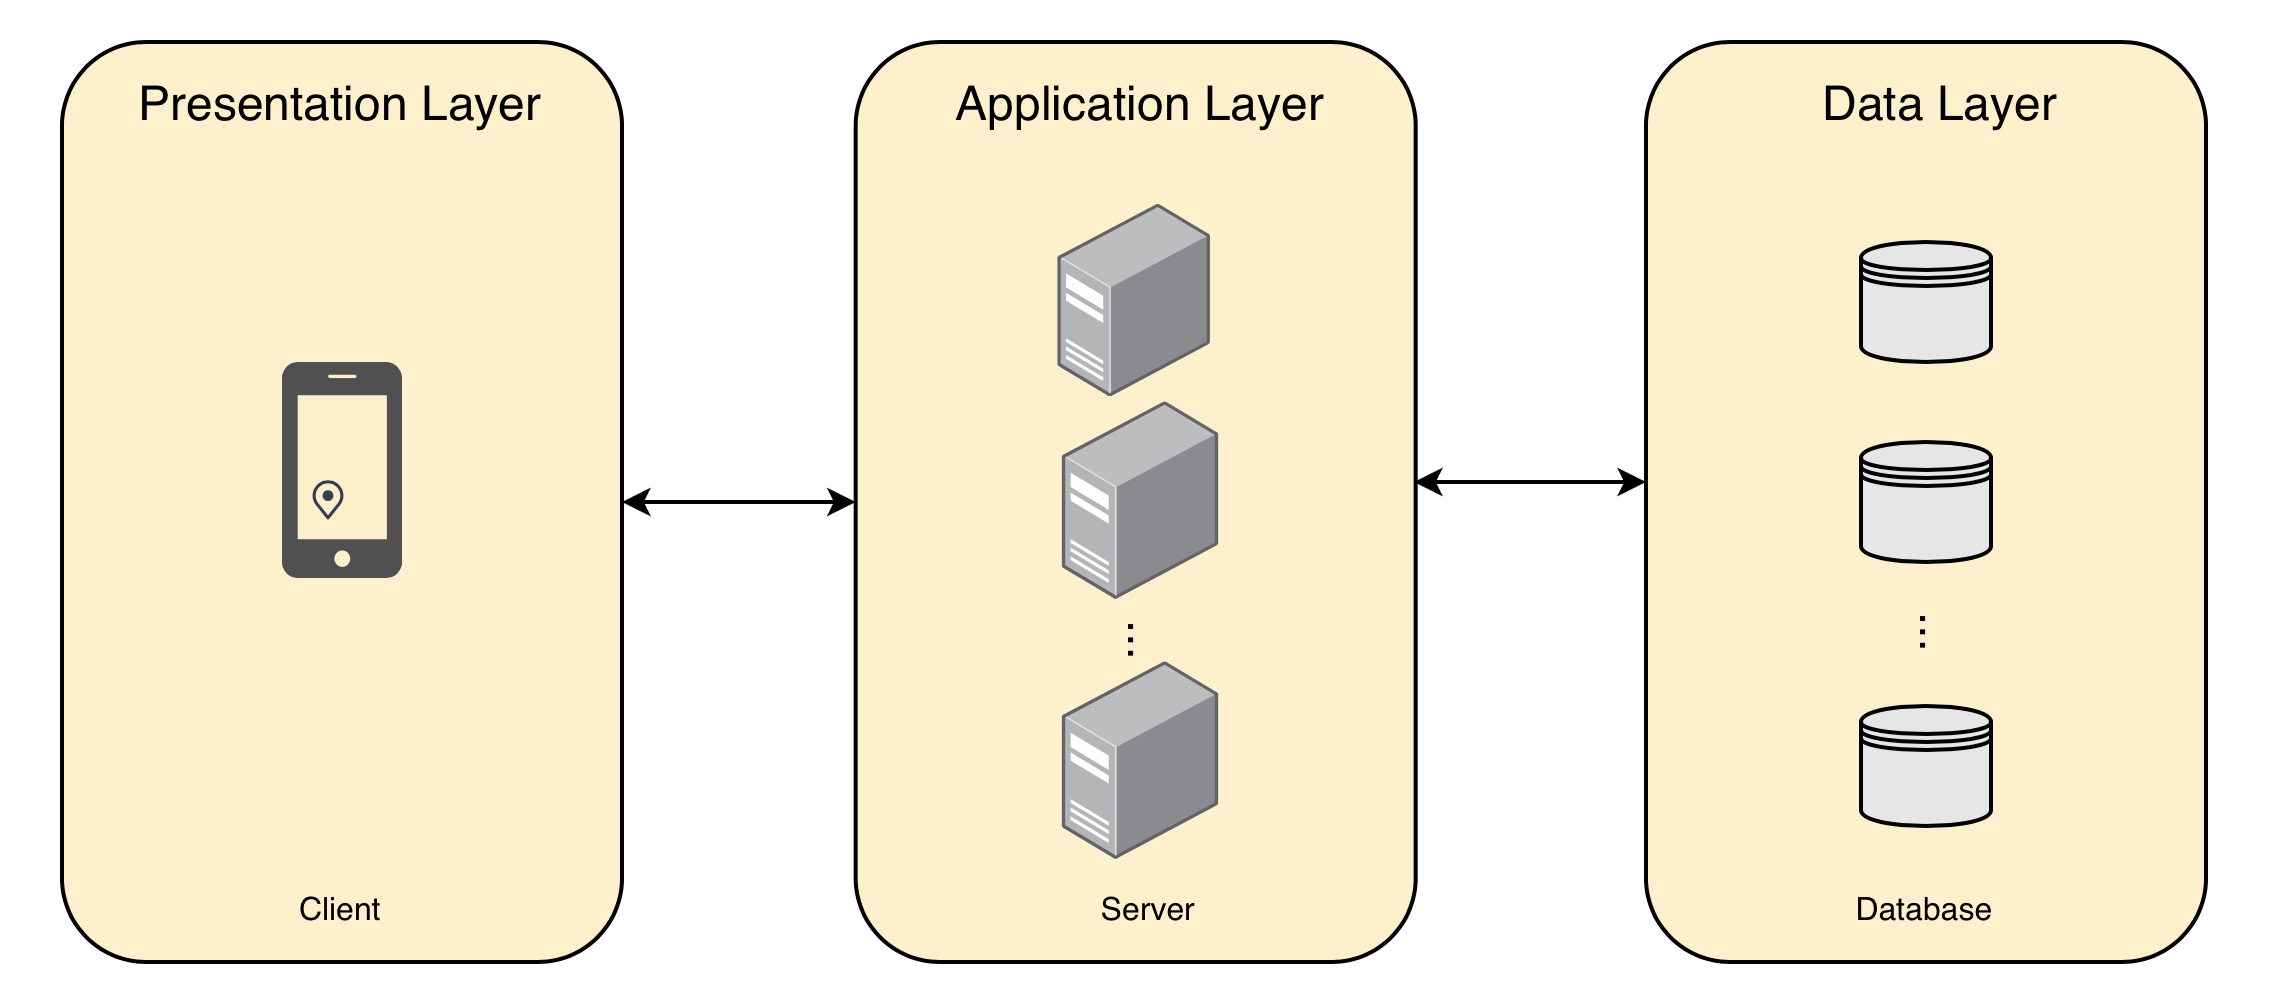
\includegraphics[width=\textwidth]{images/Architecture_Overview.png}
    \caption{High-Level Architecture Overview}
    \label{fig:high_level_architecture}
\end{figure}

\textbf{Presentation Layer}

The Presentation Layer consists of the BBP Mobile Application running on the user's mobile device (Android/iOS). The mobile app provides the user interface for authentication, trip recording, path search, and visualization. This layer also includes the embedded mobile sensors (GPS, accelerometer, gyroscope), with which the BBP application interacts through the local operating system sensor APIs to collect mobility data during automatic trip recordings.

\textbf{Application Layer}

The Application Layer implements the core business logic of the platform and is structured as a microservice-based architecture, where each service can be deployed and scaled independently. Loose coupling and improved scalability are supported by asynchronous, event-driven processing mediated by a message broker. In the deployment view, this broker is hosted on a dedicated messaging infrastructure (Messaging Tier) to isolate workloads and improve scalability and fault tolerance, while remaining part of the Application Layer from a logical perspective. Integration with external Map and Weather providers is encapsulated by dedicated adapters and safeguarded by circuit breaker mechanisms, increasing resilience against temporary outages of third-party dependencies. These architectural choices are discussed in more detail in the following sections. \\To enhance reliability and scalability, key backend components are deployed with replication, ensuring high availability and supporting higher workloads by distributing traffic and processing across multiple instances.

\textbf{Data Layer}

The Data Layer provides persistent storage for the platform and adopts a database-per-service approach to ensure clear data ownership and strong isolation between microservices. Each datastore is accessed exclusively by its corresponding service, preventing direct cross-service database access and reinforcing separation of concerns. \\To improve availability and fault tolerance, databases are deployed with replication, reducing the risk of single points of failure and supporting higher workloads by accessing redundant copies of the database.



\section{Component View}
This section describes the main software components of the BBP platform and their interactions, as illustrated in the Component Diagram. For clarity and consistency with the architectural overview, components are grouped according to the three logical layers of the system: Presentation Layer, Application Layer, and Data Layer.


\begin{figure}[H]
    \centering
    \includesvg[width=\textwidth]{images/SVG_Component_Diagram}
    \caption{Component Diagram}
    \label{fig: component_diagram}
\end{figure}


\subsection{Presentation Layer}
The Presentation Layer includes all components running on the user's mobile device and the entry point to the backend system.

The core component of this layer is the \textbf{BBP Mobile Application}, which provides the user interface for authentication, automatic and manual trip recording, trips history review, trip publication, path search and visualization. The mobile application interacts with the embedded \textbf{device sensors} (GPS, accelerometer, and gyroscope) through the local operating system sensor APIs. These sensors continuously collect mobility data, from the moment when the user starts the automatic trip recording, to the moment when it is stopped.

When the trip recording is stopped, collected sensor data are transmitted by the mobile application to the backend through the \textbf{API Gateway}, which acts as the single access point to the Application Layer. The API Gateway exposes the backend services to clients and forwards incoming requests to the appropriate internal components, enabling a clear separation between client-side logic and backend processing.

\subsection{Application Layer}
The Application Layer implements the core business logic of the platform and follows a microservice-based architectural style. Each service is responsible for a specific domain functionality and communicates asynchronously with other services.

\subsubsection{Microservices Architecture}
The backend is composed of the following microservices:

\begin{itemize}
    \item \textbf{Authentication Service} manages user registration, login, and authentication-related operations, storing credential and account data in AuthDB.
    
    \item \textbf{Trip Service} manages trip-related functionalities and stores private trip data in TripDB. It supports:
    \begin{itemize}
        \item \textbf{Manual trip recording}, where user-provided streets are processed and GPS coordinates are retrieved through the external Map service.
        \item \textbf{Automatic trip recording}, where high-frequency sensor data are ingested and persisted, immediately confirming reception after trip completion so the client can discard the transmitted trip data.
        \item \textbf{Obstacle validation}, where users accept or reject a pending obstacle on one of their private trips.
        \item \textbf{Trip publication}, allowing users to publish a private trip (for automatically recorded trips, publication is permitted only when there are no pending obstacles). When a new trip is published, the service appends an anonymized and immutable record to an append-only PublicationLog (repository stored in TripDB), ensuring that publication evidence remains even if the user later deletes the corresponding private trip.
        \item \textbf{User private history management}, enabling users to review and delete their private trips (deleting a private trip removes trip data, while the Publication Log remains). Trip trajectory is retrieved from the external Map service.
    \end{itemize}
    
    \item \textbf{Path Service}, which provides path search and visualization features. It keeps public paths state updated by applying merge results and enriches paths view with information retrieved from external Map and Weather services.
    
    \item \textbf{Analysis Service} processes automatically recorded trips to compute statistics (e.g., duration, average speed), enriching them with weather conditions if available, and detects road anomalies such as potholes. It produces obstacle candidates associated with trips and triggers the related validation workflow.
    
    \item \textbf{Merge Service} aggregates information from multiple published trips referring to the same public path. It applies merging rules and computes path scores for ranking.
\end{itemize}

\subsubsection{Message Broker and Publish/Subscribe Pattern}
To support loose coupling and asynchronous workflows, the Application Layer includes a \textbf{Message Broker} implementing a publish/subscribe (event-driven) pattern. Services publish domain events to the broker when relevant state changes occur, while other services subscribe to specific topics and react independently. This design reduces synchronous dependencies between microservices, improves scalability for background processing (analysis and merging are turned into asynchronous pipelines driven by well-defined domain events), and allows services to evolve with limited coordination.

The broker is deployed as a dedicated cluster and is responsible for reliably storing and delivering events to subscribed consumers. Events are designed to be lightweight: when data are large (e.g., high-frequency sensor streams), messages include identifiers and references to data persisted by the producing service, preventing congestion on the message bus.

The main event flows are the following:

\begin{itemize}
    \item \textbf{Trip Service} publishes \texttt{ManualTripCreated} after the creation of a manual trip and \texttt{AutomaticTripRecorded} after persisting an automatically-recorded trip (the event carries the trip identifier and references to the stored data). It also publishes \texttt{TripPublished} when a user publishes a private trip.
    
    Trip Service subscribes to \texttt{AnalysisCompleted} (from Analysis Service) that triggers statistics update inside the TripDB.
    
    \item \textbf{Analysis Service} subscribes to \texttt{AutomaticTripRecorded} (from Trip Service) to compute trip statistics and detect anomalies. It publishes \texttt{AnalysisCompleted} as soon as the analysis is completed. It does not access TripDB directly, relying on events and references produced by Trip Service.
    
    \item \textbf{Merge Service} subscribes to \texttt{TripPublished} to aggregate contributions and compute/update the path score, then publishes \texttt{MergeCompleted}, containing the merge outcome and updated scoring information. Merge Service does not access PathDB directly: it produces merge results as events later consumed by Path Service.
    
    \item \textbf{Path Service} subscribes to \texttt{MergeCompleted} and applies merge results to update PathDB, keeping path status and ranking consistent with the latest published information.
\end{itemize}

\subsubsection{External Services Integration}
The platform integrates with external Map and Weather services to enrich path computation and trip analysis. Access to these third-party services is encapsulated by dedicated \textbf{service adapters}, which isolate external APIs from the core application logic.

Each adapter is protected by a \textbf{Circuit Breaker} mechanism to prevent cascading failures and to improve resilience against slow responses, latency spikes, or temporary unavailability of external providers.

\subsection{Data Layer}
The Data Layer is responsible for persistent data storage and follows a \textbf{database-per-service} pattern to ensure strong data ownership and isolation. Each microservice can access only its own datastore, preventing direct cross-service database access and reinforcing separation of concerns.

\begin{itemize}
    \item \textbf{Authentication Service} interacts exclusively with AuthDB, a relational database storing user credentials and authentication-related data.
    
    \item \textbf{Path Service} interacts exclusively with PathDB, a relational database containing public paths information.
    
    \item \textbf{Trip Service} interacts exclusively with TripDB, which is implemented as a time-series database to efficiently store high-frequency sensor data collected during trips.
    \begin{itemize}
        \item During an automatically recorded trip, the mobile application continuously collects sensor data and, when the user stops the recording, sends the recorded trip data through the API Gateway to the Trip Service. The Trip Service immediately acknowledges successful reception so the client can safely discard the transmitted batches, and then it persists ingested trip data into the TripDB. This approach enables efficient handling of high-volume time-series streams while preserving a clear and controlled data flow from the client to persistent storage.
        \item Within TripDB, the Trip Service also maintains an append-only PublicationLog containing anonymized records of published trips: this log is immutable and persists independently from private trip data, which may be deleted by the user.
    \end{itemize}
\end{itemize}

\section{Deployment Diagram}
This section describes the physical deployment of the BBP platform, illustrating how software components are mapped onto hardware nodes and infrastructure elements.

\begin{figure}[H]
    \centering
    \includesvg[width=\textwidth]{images/Deployment_Diagram.svg}
    \caption{Deployment Diagram}
    \label{fig: cdeployment_diagram}
\end{figure}

\begin{itemize}
    \item \textbf{Client Tier} consists of the users' mobile devices (Android/iOS), which host the BBP Mobile Application and embedded device sensors (GPS, accelerometer, gyroscope). The mobile application interacts locally with sensors through operating system APIs and communicates remotely with the backend using HTTPS.
    
    All outbound client traffic is filtered by a Firewall, which allows inbound HTTPS connections exclusively to the API Gateway, protecting data and application layers from potential threats.
    
    \item \textbf{Application Tier} hosts the core backend infrastructure and is deployed on an Application Server cluster. Client requests first pass through a Load Balancer, which distributes traffic across multiple replicated instances of the API Gateway (2..N) to ensure scalability and availability. Behind the API Gateway, each service (Authentication, Trip, Path, Analysis, and Merge) is deployed in replicated execution environments (2..N). Internal components, labeled as LB, represent service-specific load balancers that distribute requests received from the API Gateway across the available replicas of each microservice. Integration with external Map and Weather providers is handled through a dedicated Adapter Layer, where each adapter is protected by a Circuit Breaker (CB) mechanism to improve resilience against slow responses or temporary unavailability of third-party services.
    
    Notes:
    \begin{itemize}
        \item External services are assumed to include their own security and firewall mechanisms and are therefore not detailed further in the diagram.
        \item For readability, the Deployment Diagram omits the explicit representation of the \texttt{<<artifact>>} elements contained within each service execution environment.
    \end{itemize}
    
    \item \textbf{Messaging Tier} is deployed as a separate cluster and provides the asynchronous event bus of the system. It consists of multiple Broker Nodes (3..N) hosting the Message Broker execution environment.
    
    Communication between the Application Tier and the Messaging Tier is protected by a Firewall, which allows only broker-specific protocol ports, preventing unauthorized access. All publish/subscribe interactions are represented as bidirectional communication links, reflecting that services both publish events and consume them asynchronously.
    
    \item \textbf{Data Tier} is deployed as a Database Server Cluster (3..N) and follows a database-per-service pattern to enforce strict data ownership and isolation. Each microservice can access only its corresponding database, and no lateral database access is allowed. This isolation is enforced through a Firewall placed between the Application Tier and the Data Tier, with three distinct logical connections, one per database. Each connection allows only the required database ports from the corresponding service subnet, explicitly denying cross-service access.
    
    The adopted database technologies are:
    \begin{itemize}
        \item \textbf{AuthDB:} relational DBMS for authentication and user data
        \item \textbf{PathDB:} relational DBMS for public paths and rankings
        \item \textbf{TripDB:} time-series database optimized for high-frequency sensor data collected during trips
    \end{itemize}
    
    All databases are deployed with replication (1..N replicas) to improve fault tolerance, availability, and read scalability.
\end{itemize}

\section{Runtime View}
\label{sec:runtime-view}
% Testo introduttivo
For the sake of visual clarity and to avoid diagrammatic clutter, the API Gateway lifeline has been omitted from all of the sequence diagrams. Architecturally, however, it mediates all interactions between the Client and the Backend services and routes requests to the appropriate microservice without altering the core business logic.

% --------------------------------------------------------
% 1. User Sign Up
% --------------------------------------------------------
\subsection{User Sign Up}
The process initiates when the User submits registration details via the BBP Mobile App. The request is routed to the Auth Service, which validates the input syntax and performs security checks (e.g., password hashing). Upon verification, the service persists the new user identity into the Auth DB. Finally, a confirmation message is returned to the client, providing immediate feedback on the successful account creation.

\begin{figure}[H]
    \centering
    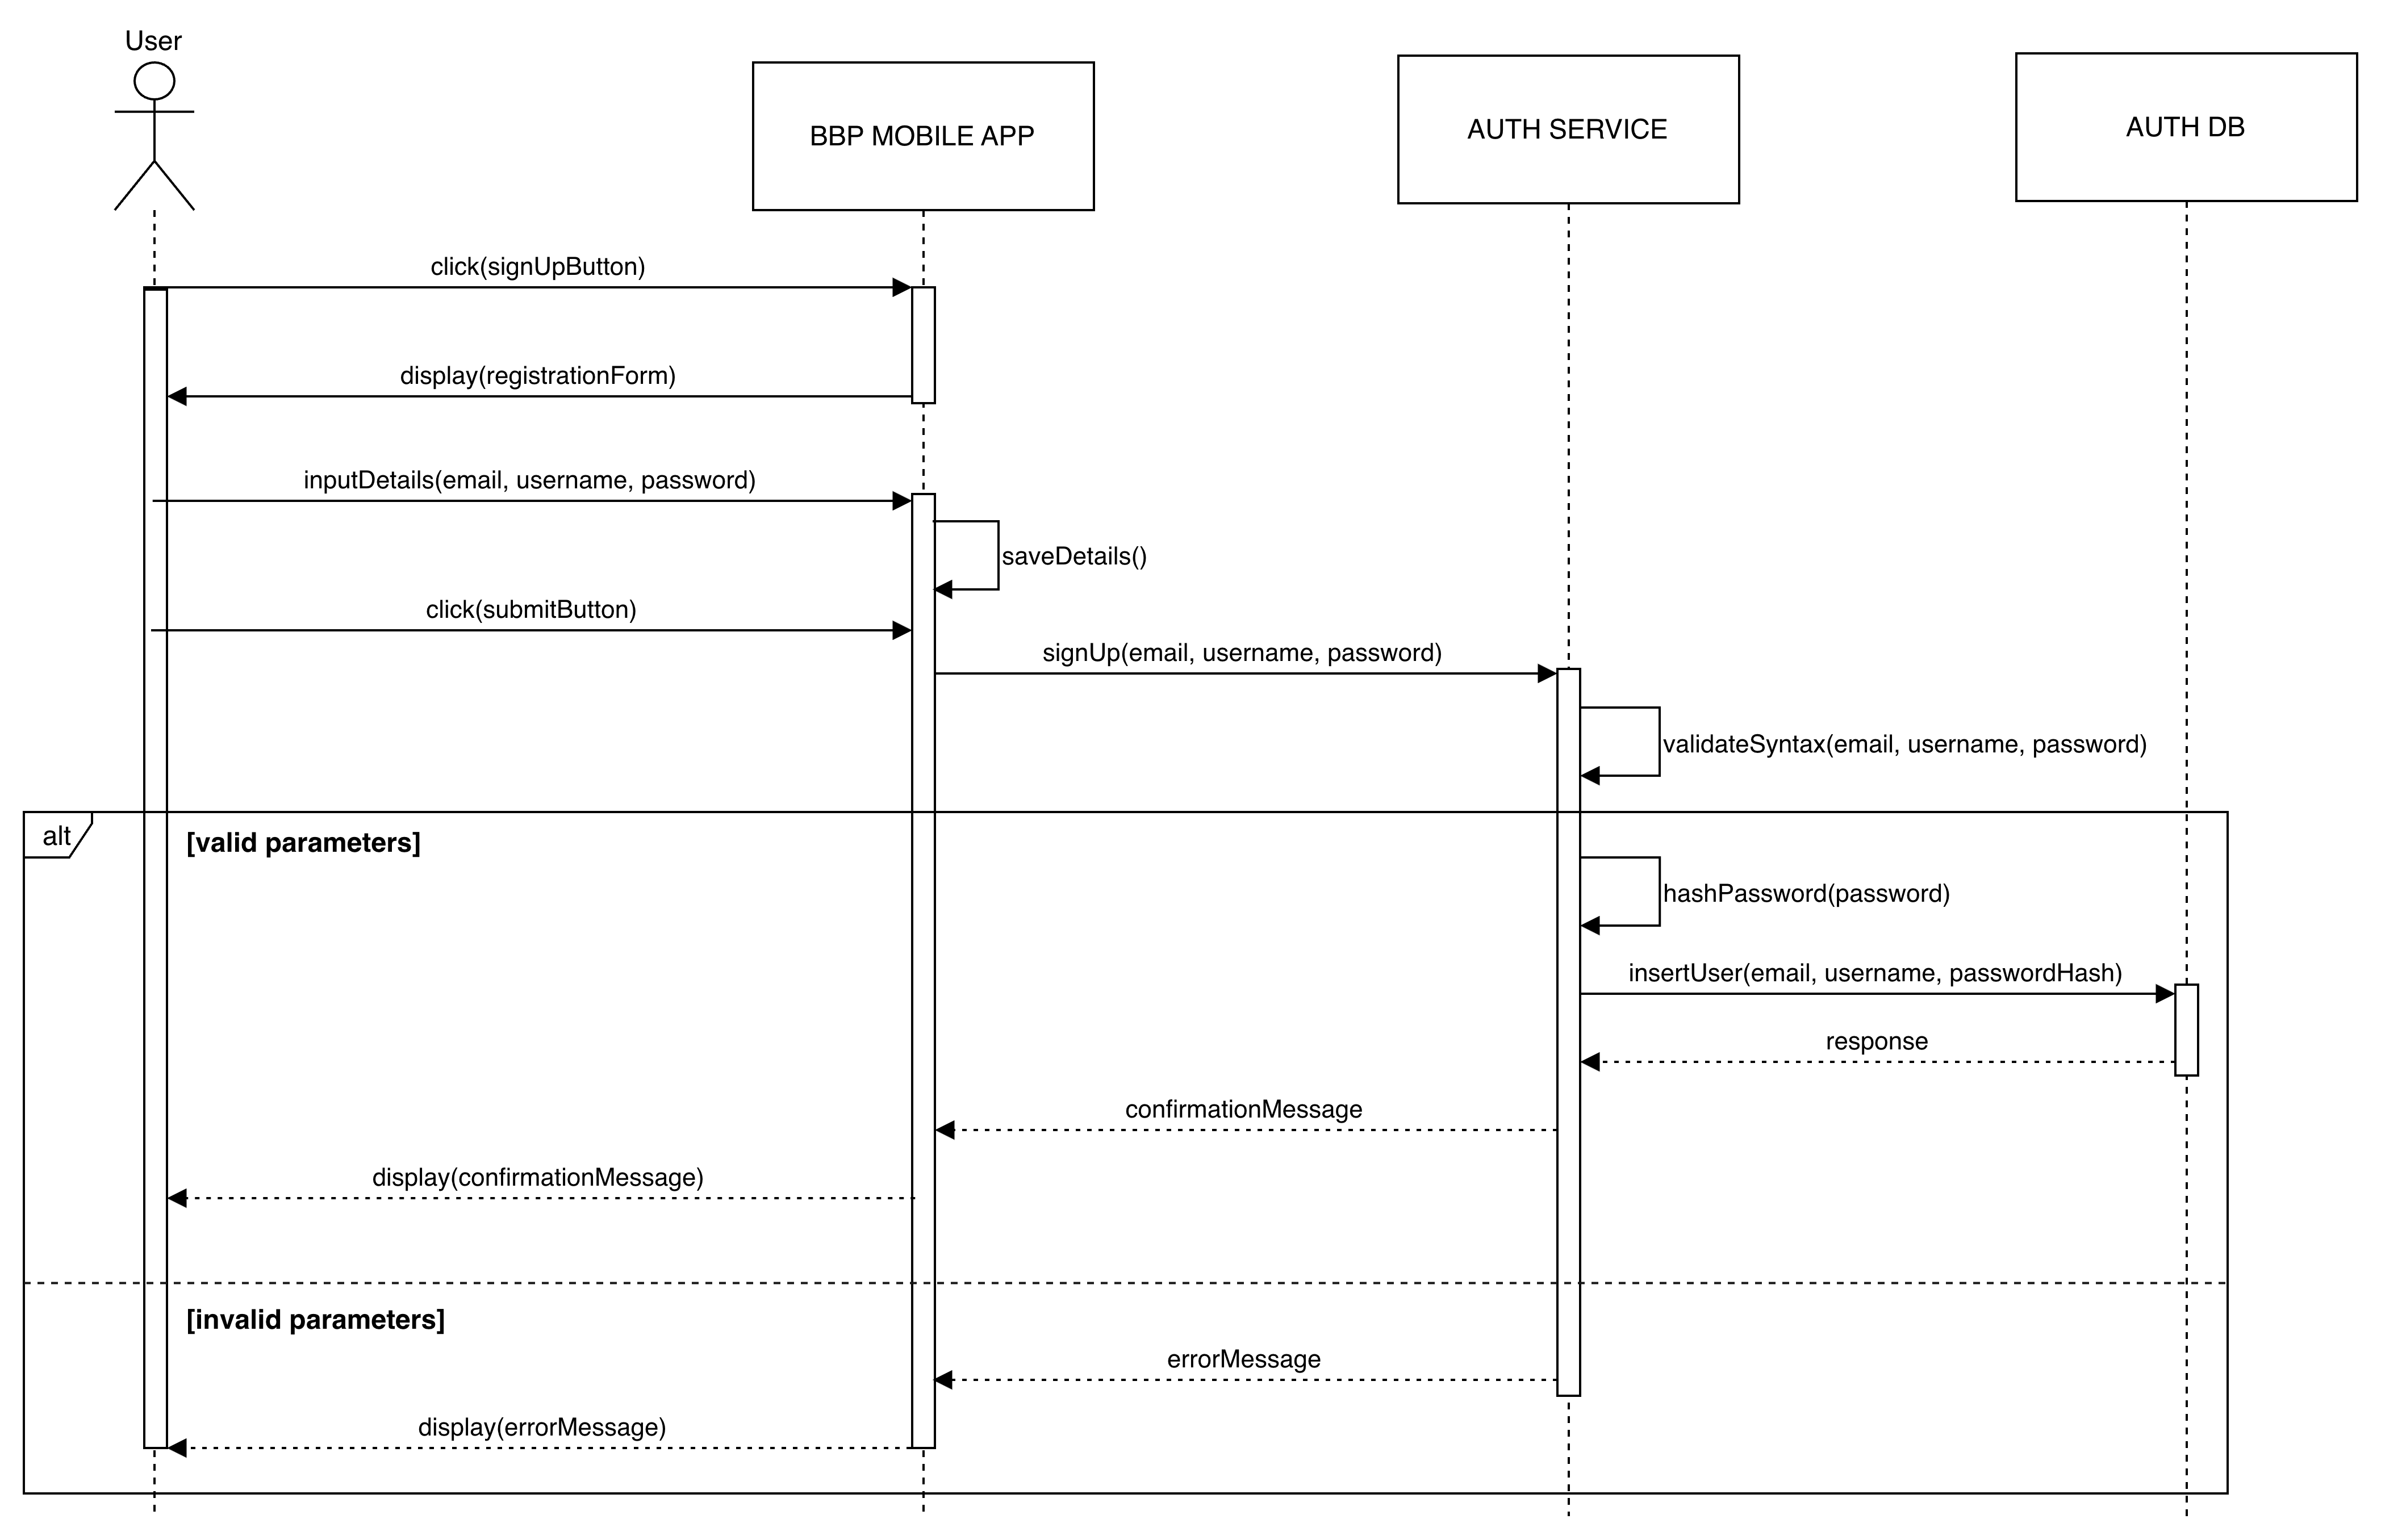
\includegraphics[width=\textwidth]{DD/images/runtime_views/rv1_signup.png}
    \caption{Sequence Diagram: User Sign Up}
    \label{fig:seq_signup}
\end{figure}

% --------------------------------------------------------
% 2. User Log In
% --------------------------------------------------------
\subsection{User Log In}
The login flow begins with the User entering credentials in the BBP Mobile App. The Auth Service receives the request and queries the Auth DB to verify the username and password hash. If valid, the service generates a session token and returns it within a success response. The client application stores this token locally to authorize subsequent API requests, ensuring a stateless authentication mechanism.

\begin{figure}[H]
    \centering
    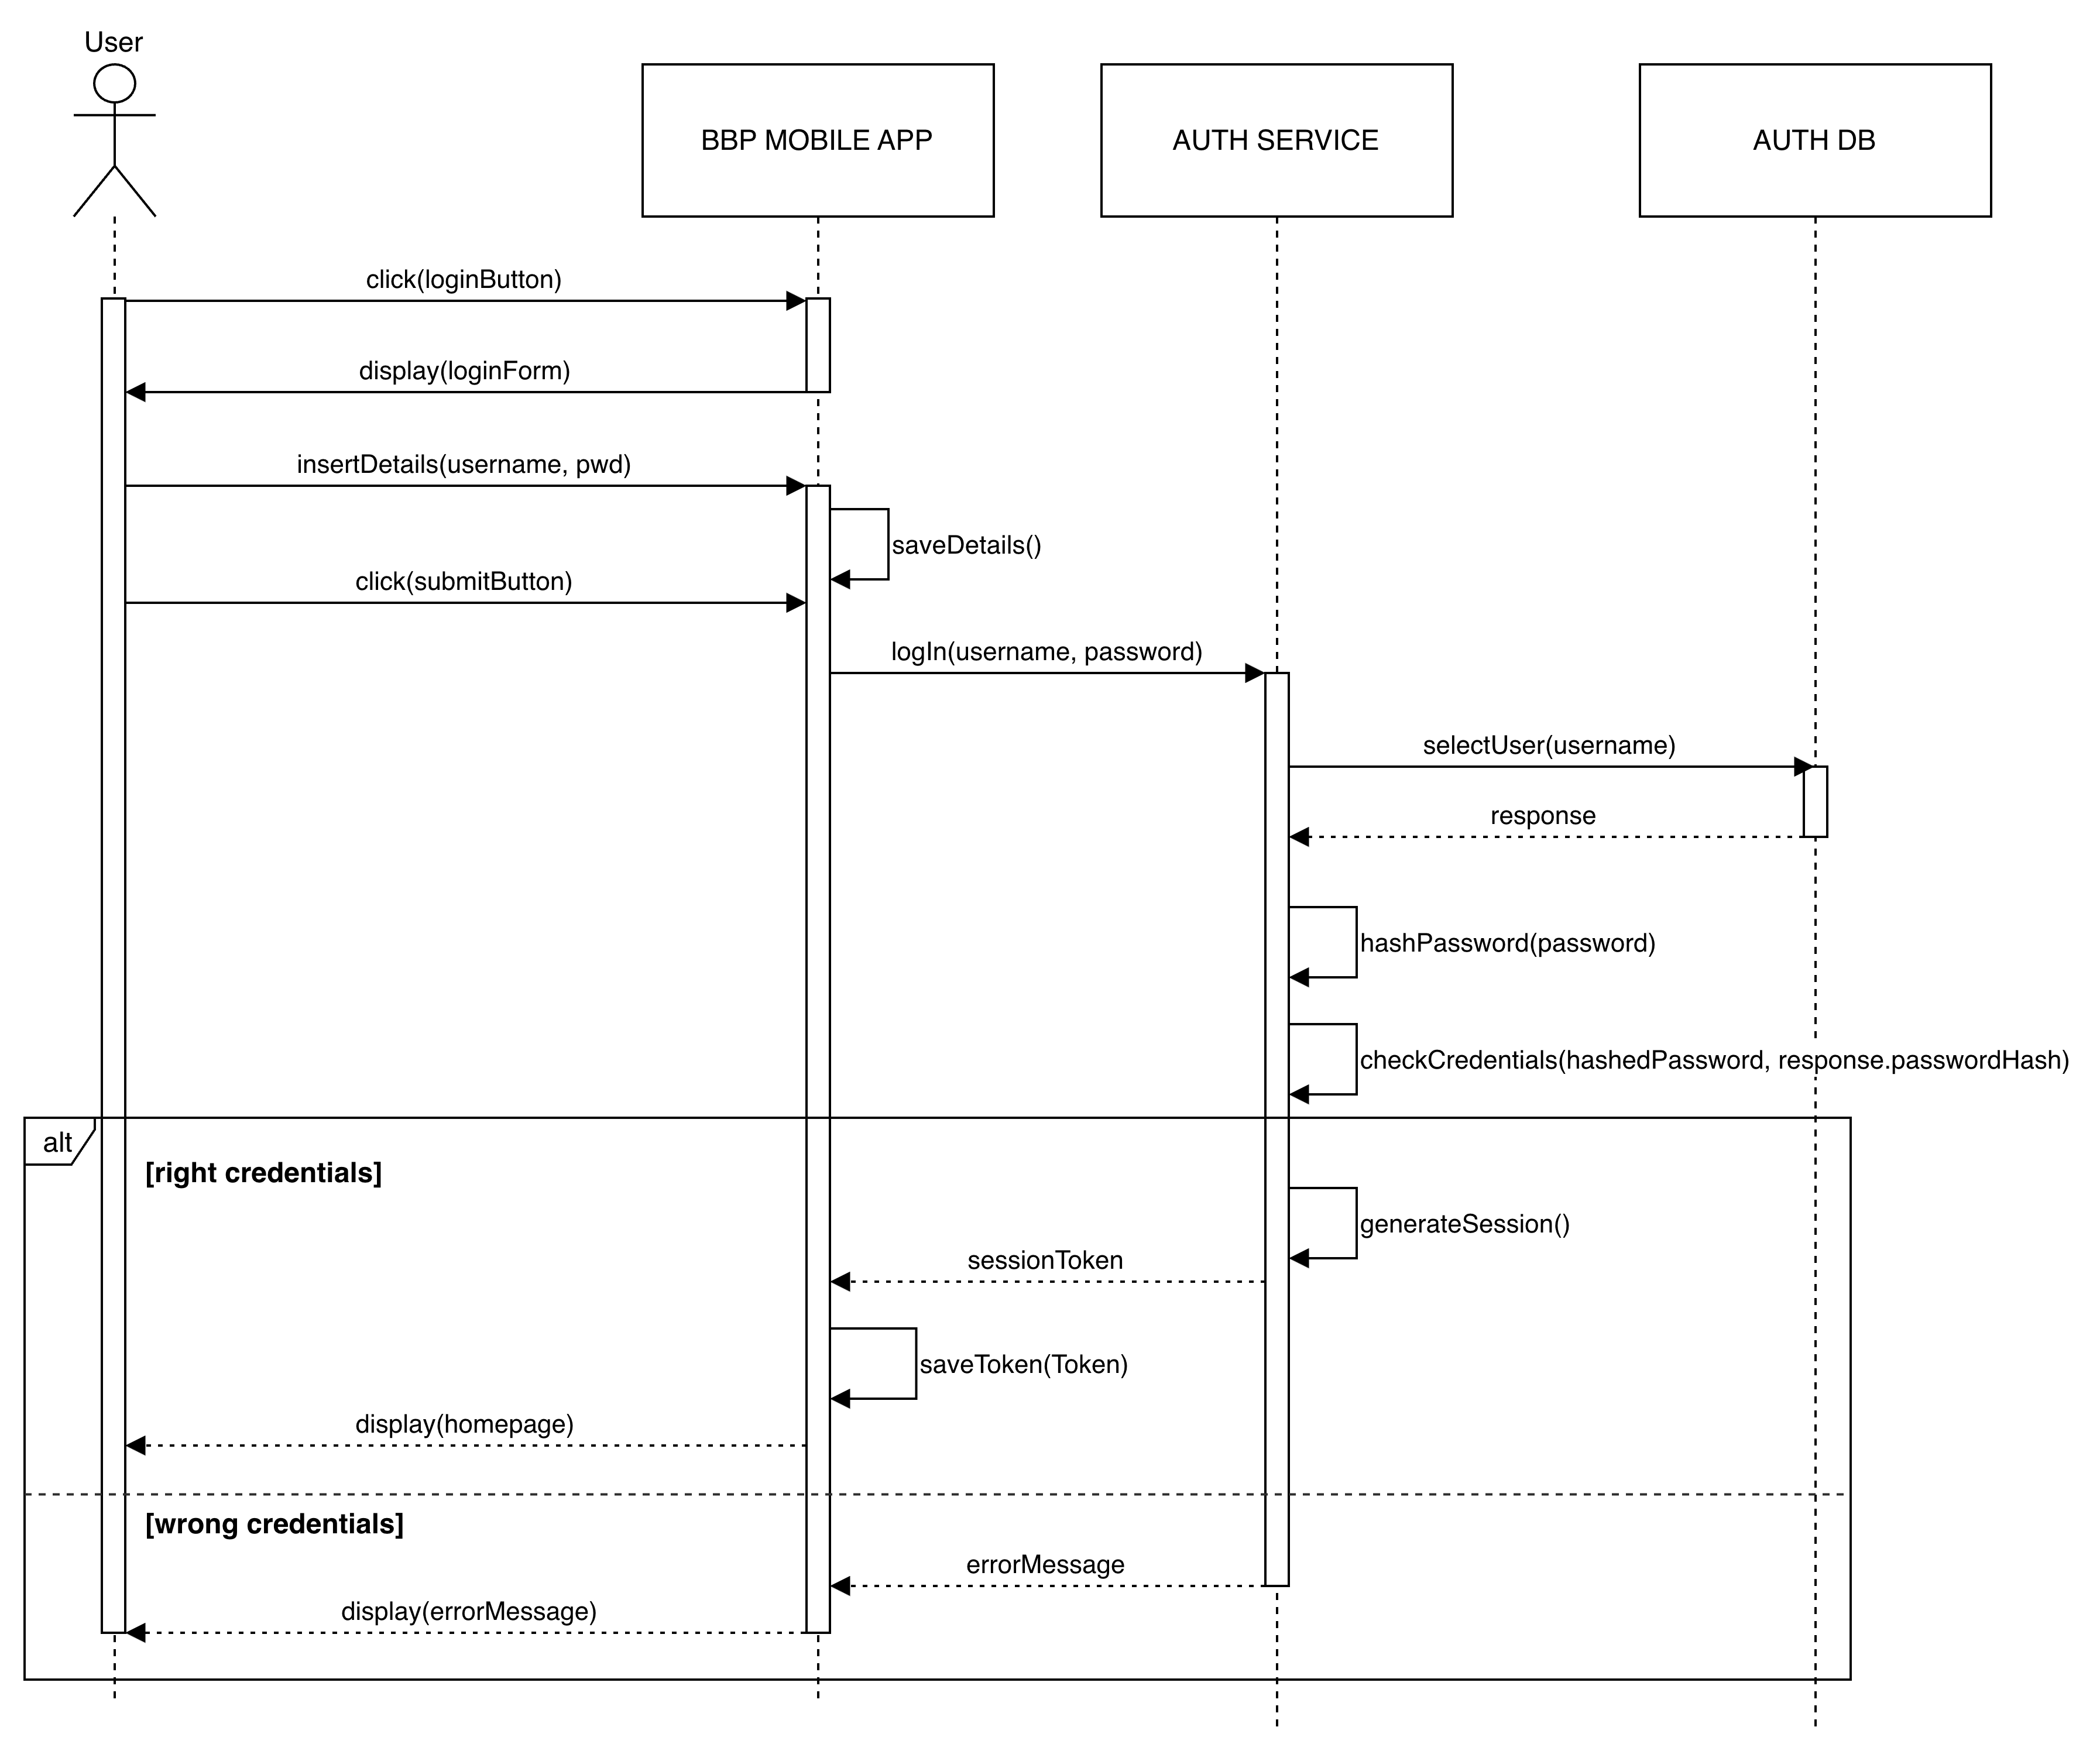
\includegraphics[width=\textwidth]{DD/images/runtime_views/rv2_login.png}
    \caption{Sequence Diagram: User Log In}
    \label{fig:seq_login}
\end{figure}

% --------------------------------------------------------
% 3. Automatic Recording
% --------------------------------------------------------
\subsection{Automatic Recording}
Recording initiates when the Mobile App detects movement exceeding a speed threshold. The App enters a loop, batching sensor data (GPS) and storing it locally. Upon session termination, the service finalizes the transaction sending the locally saved data to the database and produces an \texttt{automaticTripRecorded} event to the Message Broker to trigger asynchronous analysis.

\begin{figure}[H]
    \centering
    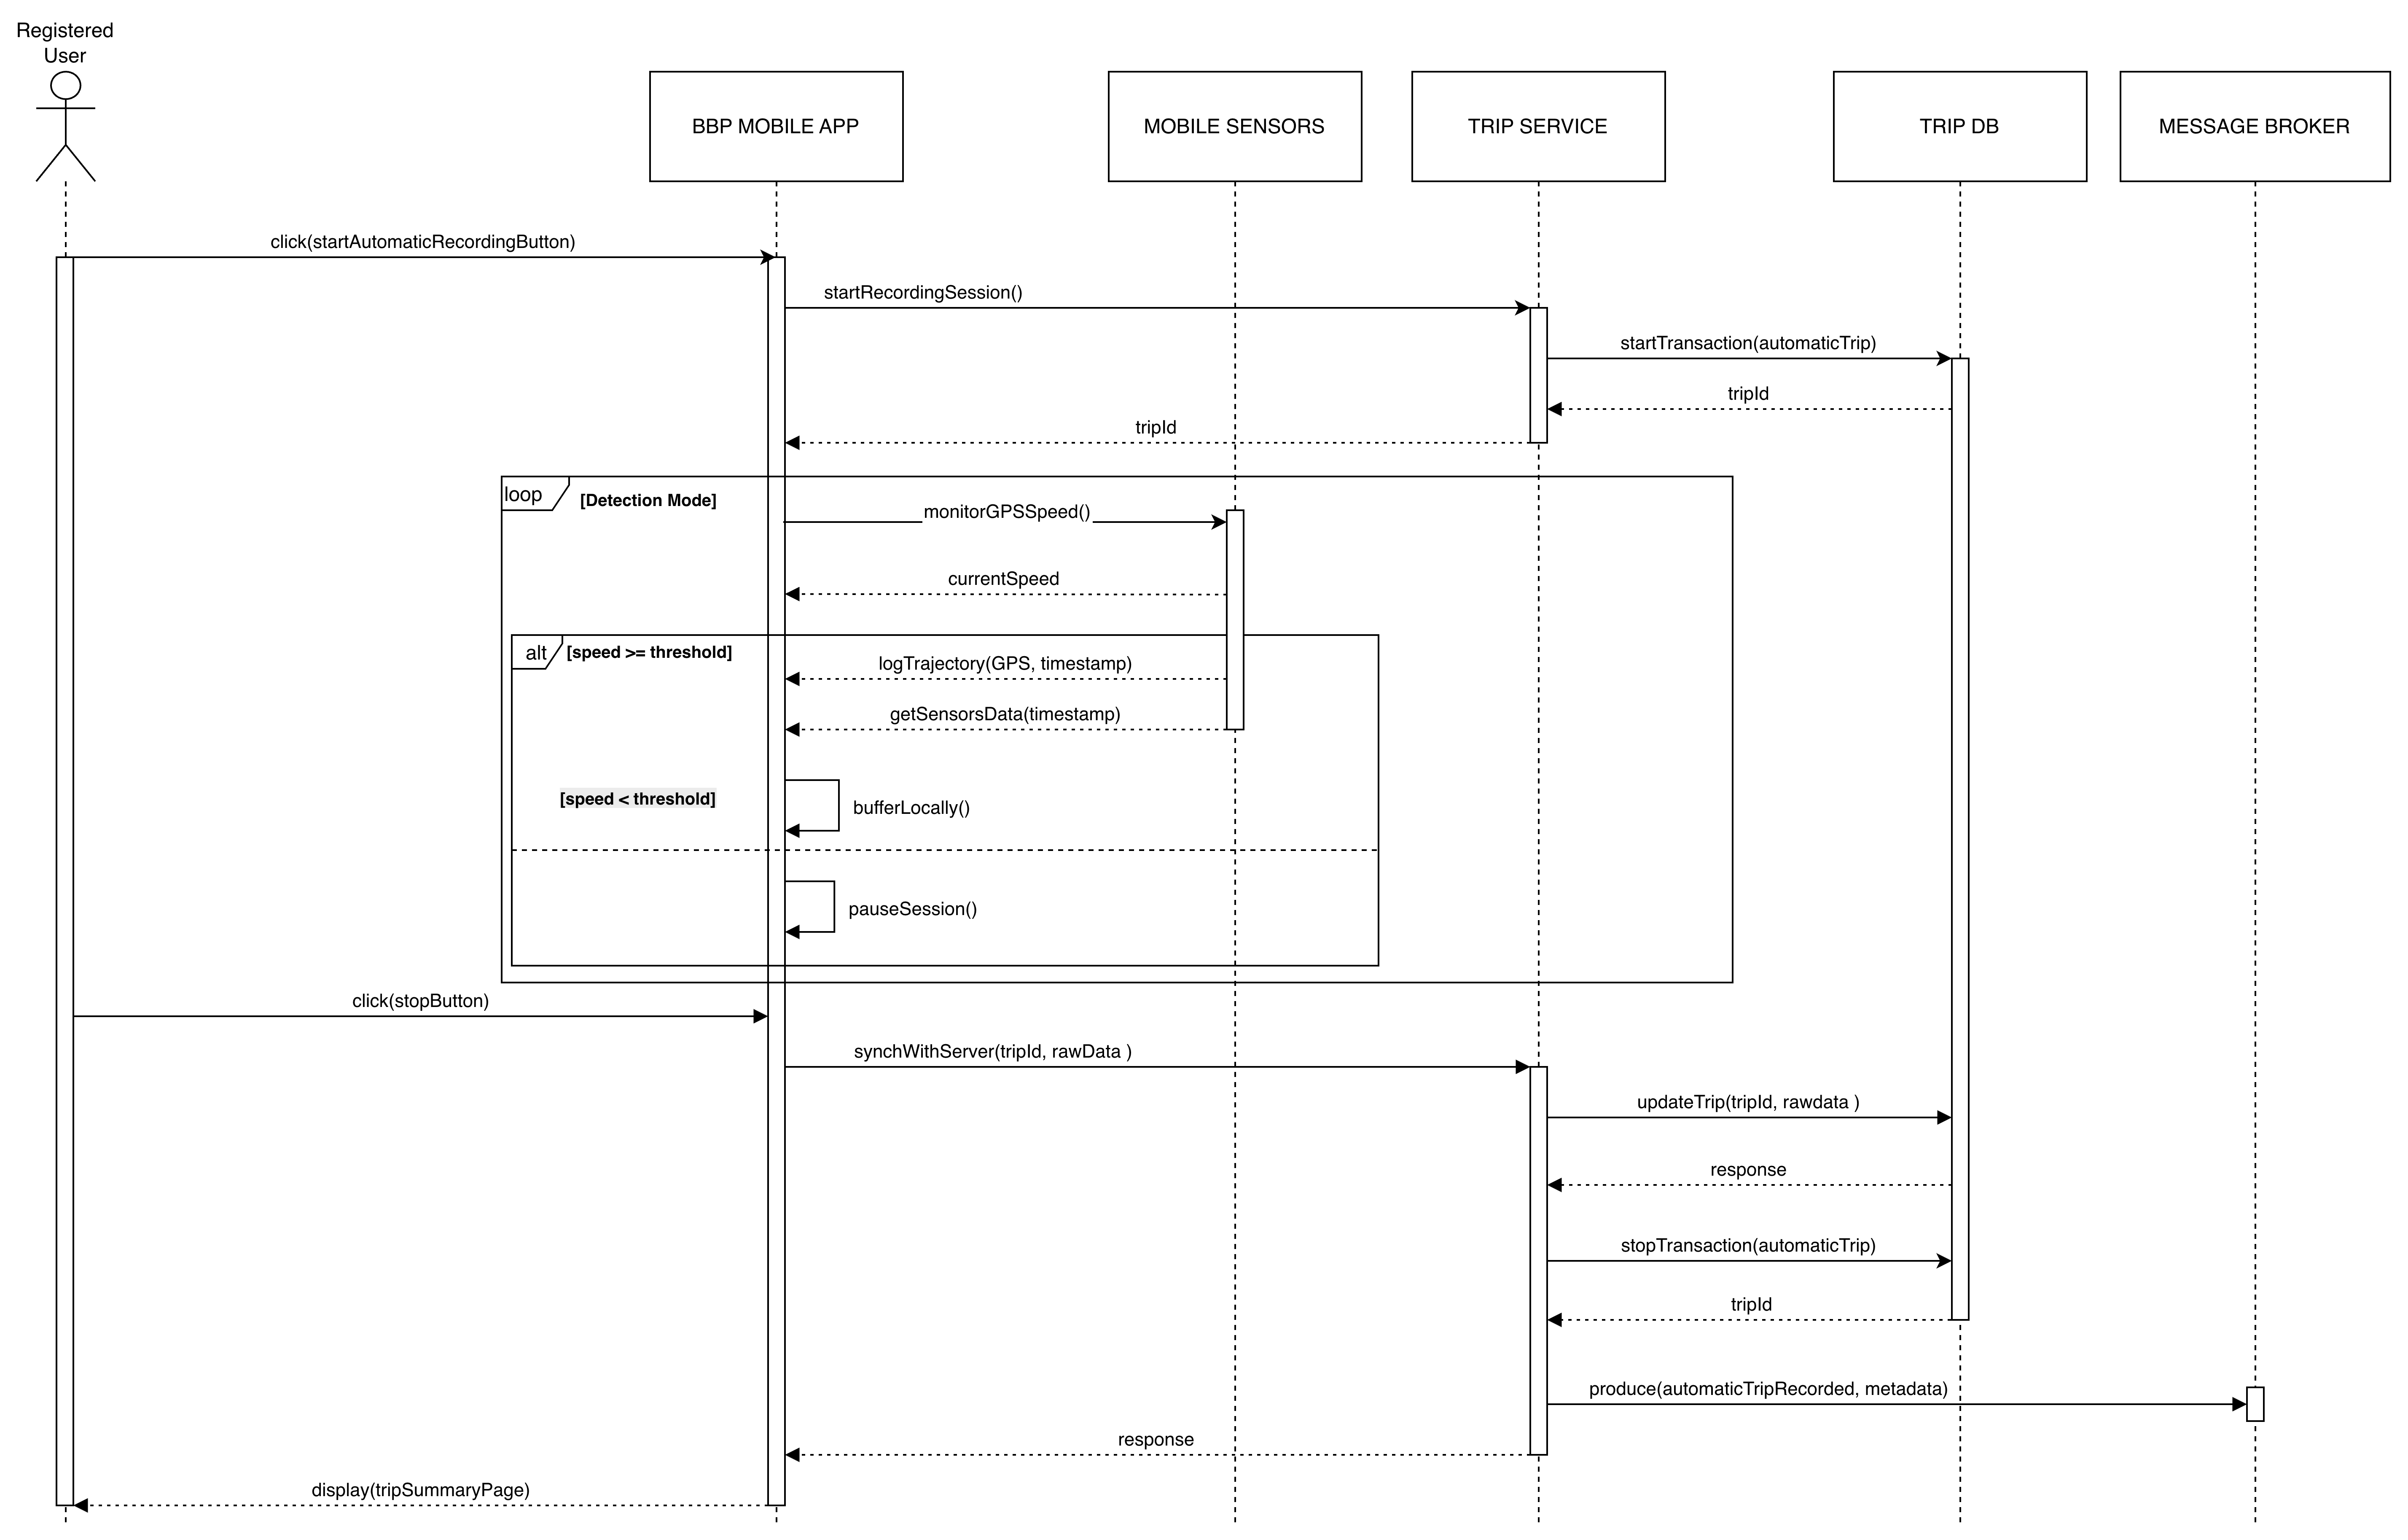
\includegraphics[width=\textwidth]{DD/images/runtime_views/rv3_automatic_recording.png}
    \caption{Sequence Diagram: Automatic Recording}
    \label{fig:seq_automatic_recording}
\end{figure}

% --------------------------------------------------------
% 4. Manual Recording and Insert Street Entry
% --------------------------------------------------------
\subsection{Manual Recording and Insert Street Entry}
The Registered User manually builds a trip by inserting street entries (UC4.1). For every entry, the Trip Service validates the street name in real-time by querying the Map Service Adapter (safeguarded by the Circuit Breaker pattern). Once the user confirms the full list of streets, the service persists the trip in the Trip DB and publishes a \texttt{manualTripCreated} event to the Message Broker.

\textbf{Circuit Breaker Implementation:} Crucially, the synchronous interaction with the external Map Provider is protected by the Circuit Breaker pattern. This mechanism monitors the adapter for timeouts or failures. If the error rate exceeds a threshold, the circuit "opens" to fail-fast, preventing resource exhaustion and ensuring the backend remains responsive even during third-party service outages.

\begin{figure}[H]
    \centering
    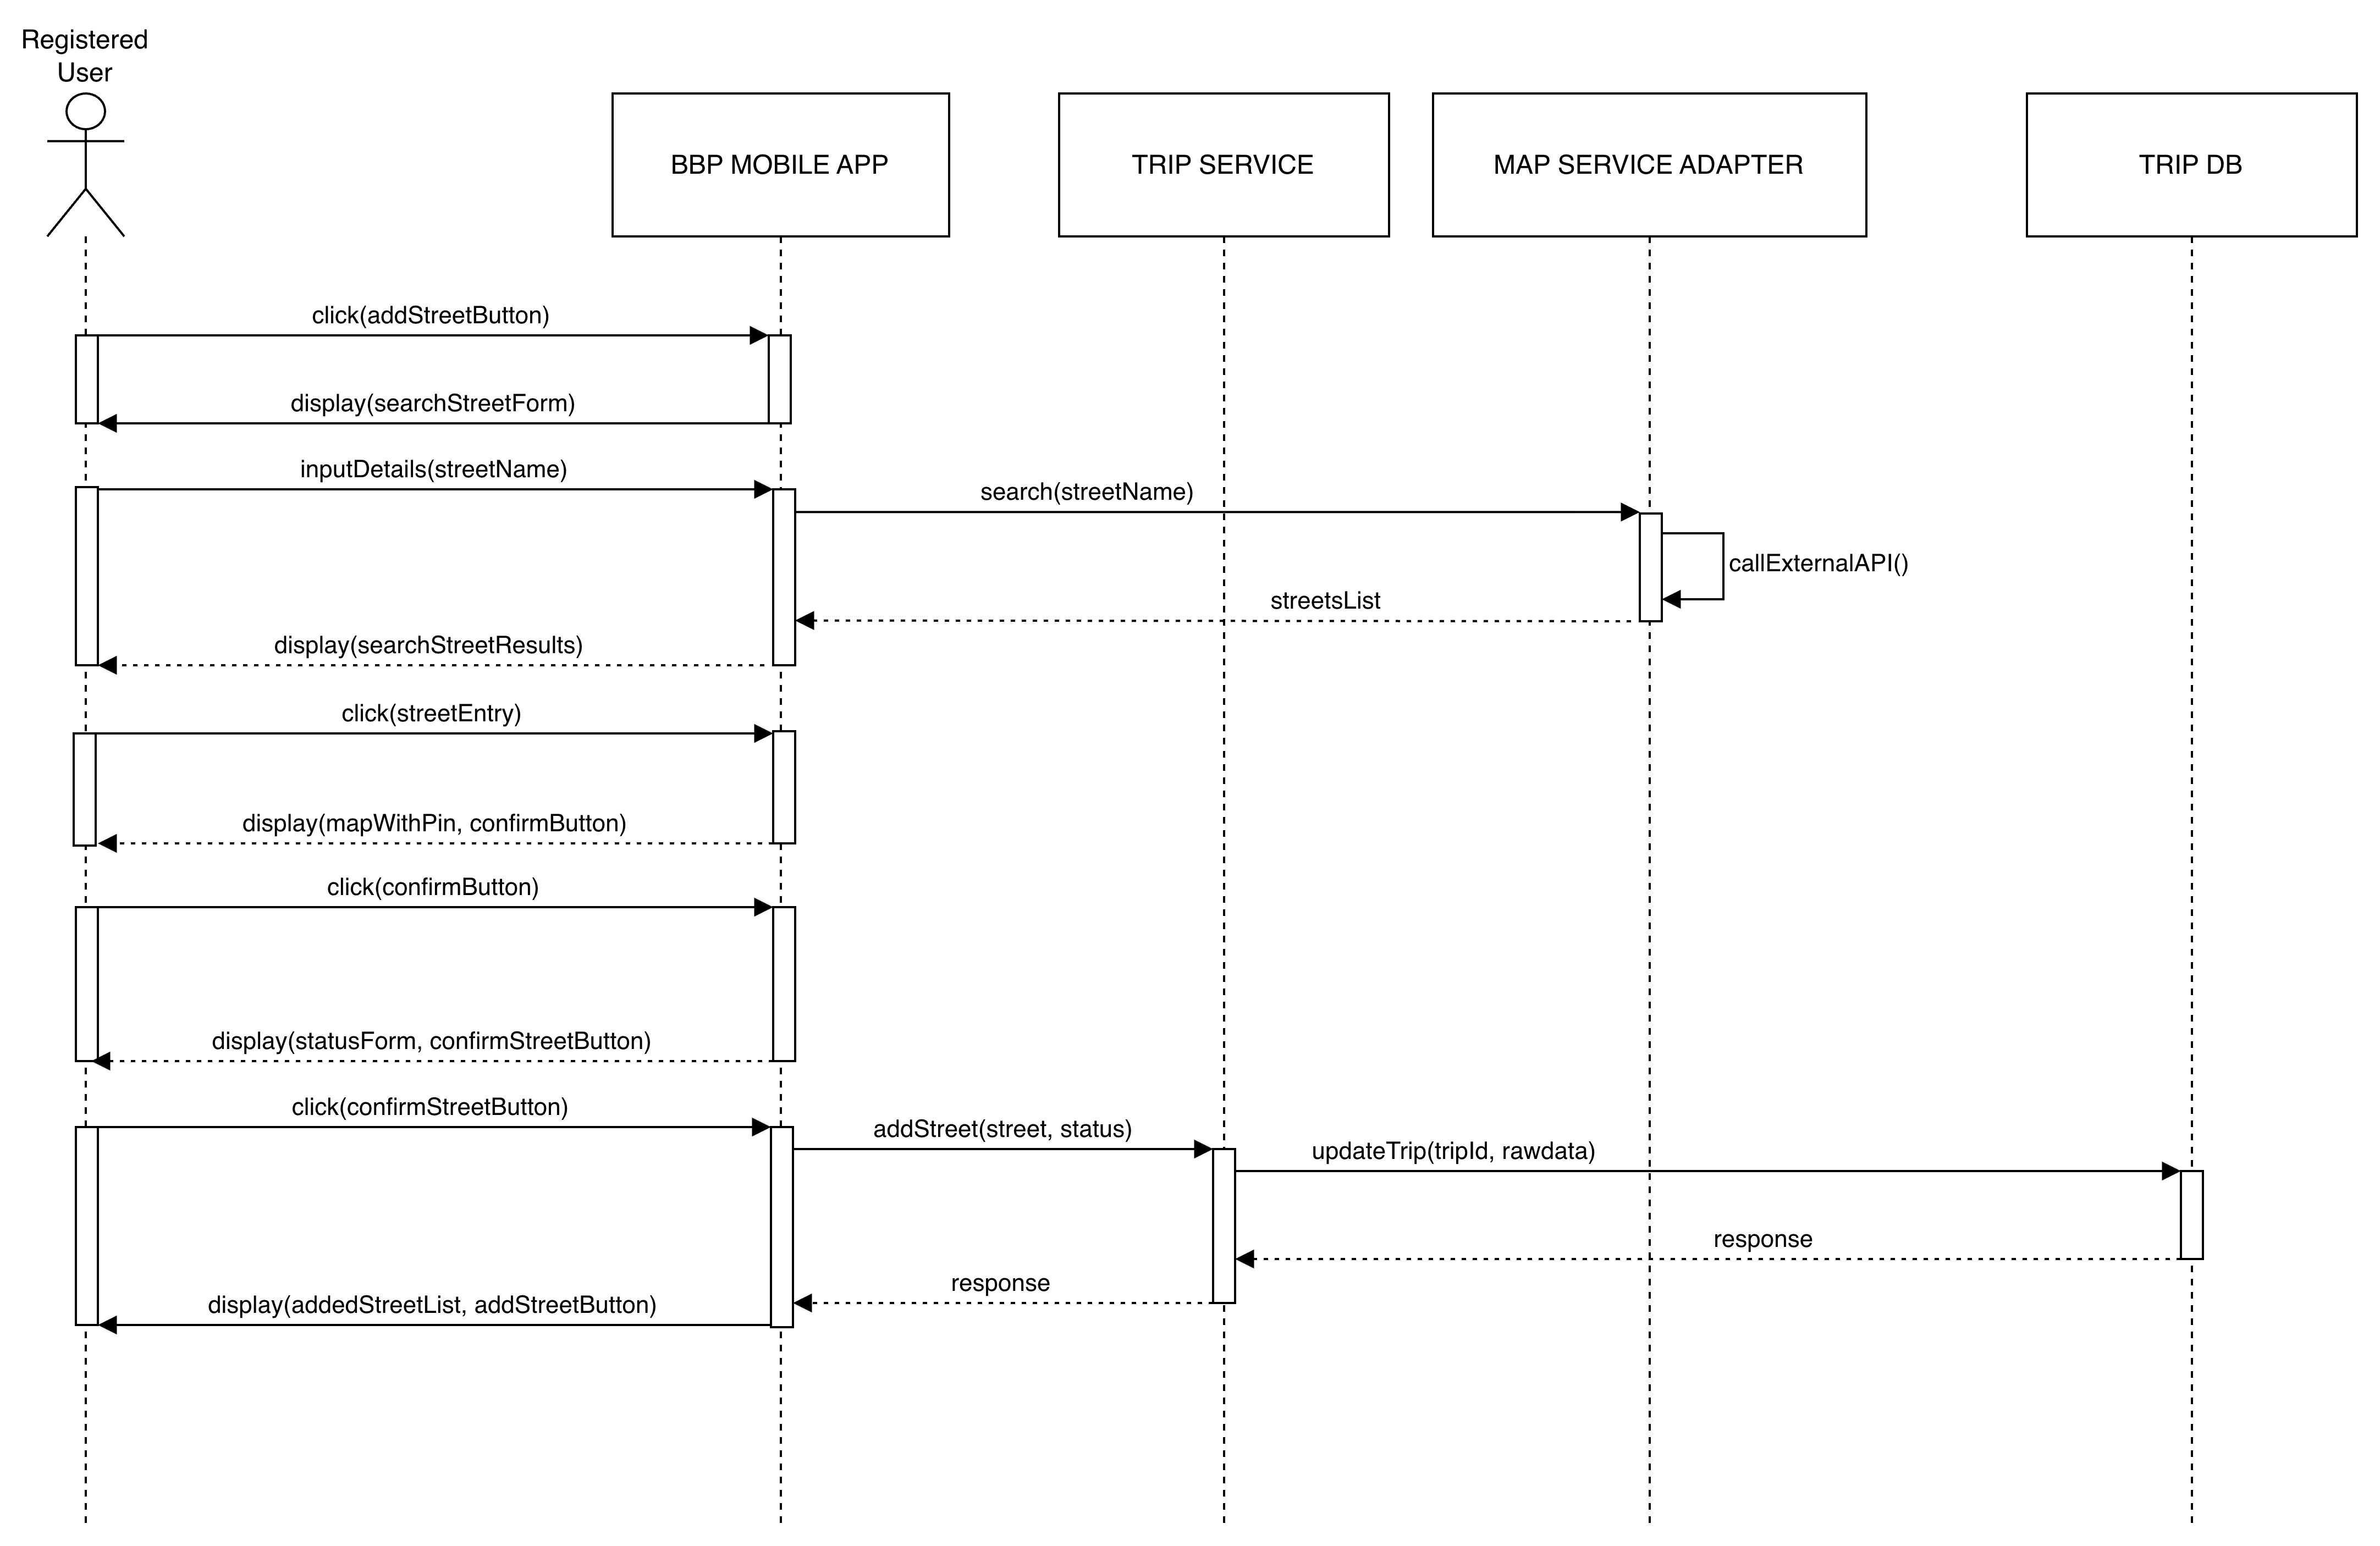
\includegraphics[width=\textwidth]{DD/images/runtime_views/rv4_0_insert_street_entry.png}
    \caption{Sequence Diagram: Insert Street Entry}
    \label{fig:seq_manual_recording}
\end{figure}
\begin{figure}[H]
    \centering
    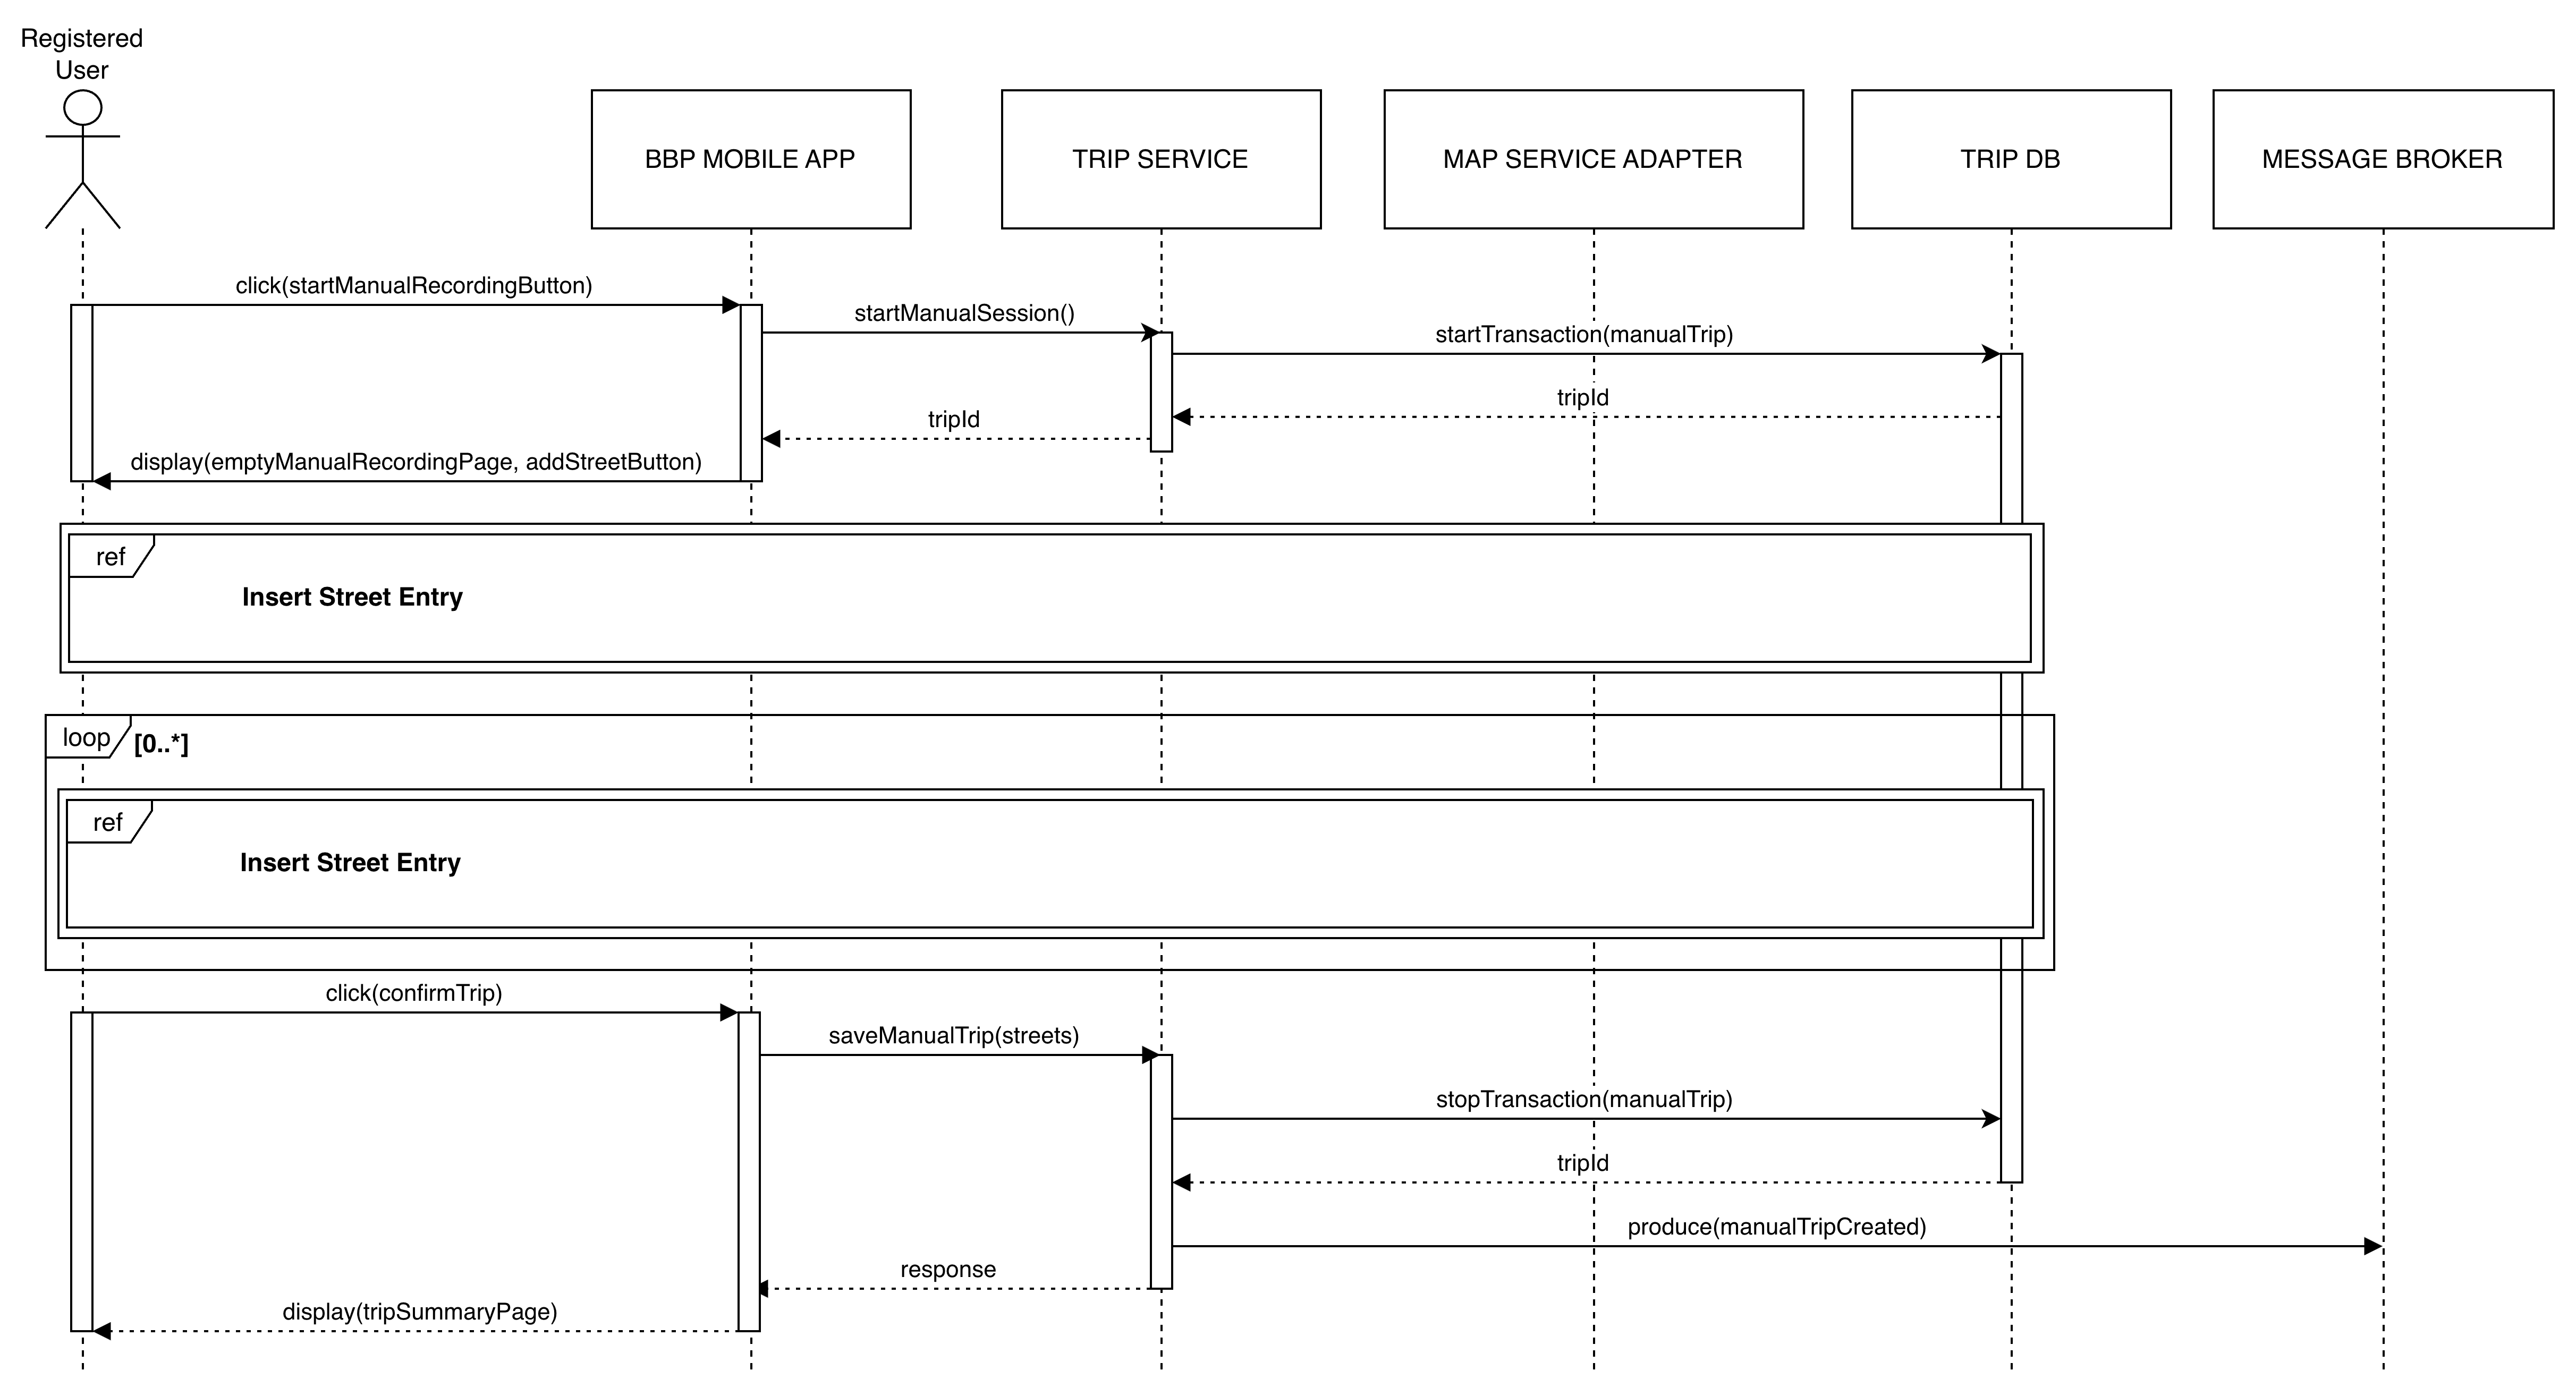
\includegraphics[width=\textwidth]{DD/images/runtime_views/rv4_manual_recording.png}
    \caption{Sequence Diagram: Manual Recording}
    \label{fig:seq_manual_recording}
\end{figure}

% --------------------------------------------------------
% 5. Validate Obstacles
% --------------------------------------------------------
\subsection{Validate Obstacles}
To validate anomalies, the Trip Service retrieves trip metadata from the Trip DB and fetches the visual trajectory via the Map Service Adapter (protected by the Circuit Breaker). The User iterates through pending anomalies on the Mobile App, accepting or rejecting each. These decisions are sent synchronously to the Trip Service, which updates the anomaly status in the Trip DB. Once all anomalies are handled and the status of the path is provided, the trip is marked as validated.

\begin{figure}[H]
    \centering
    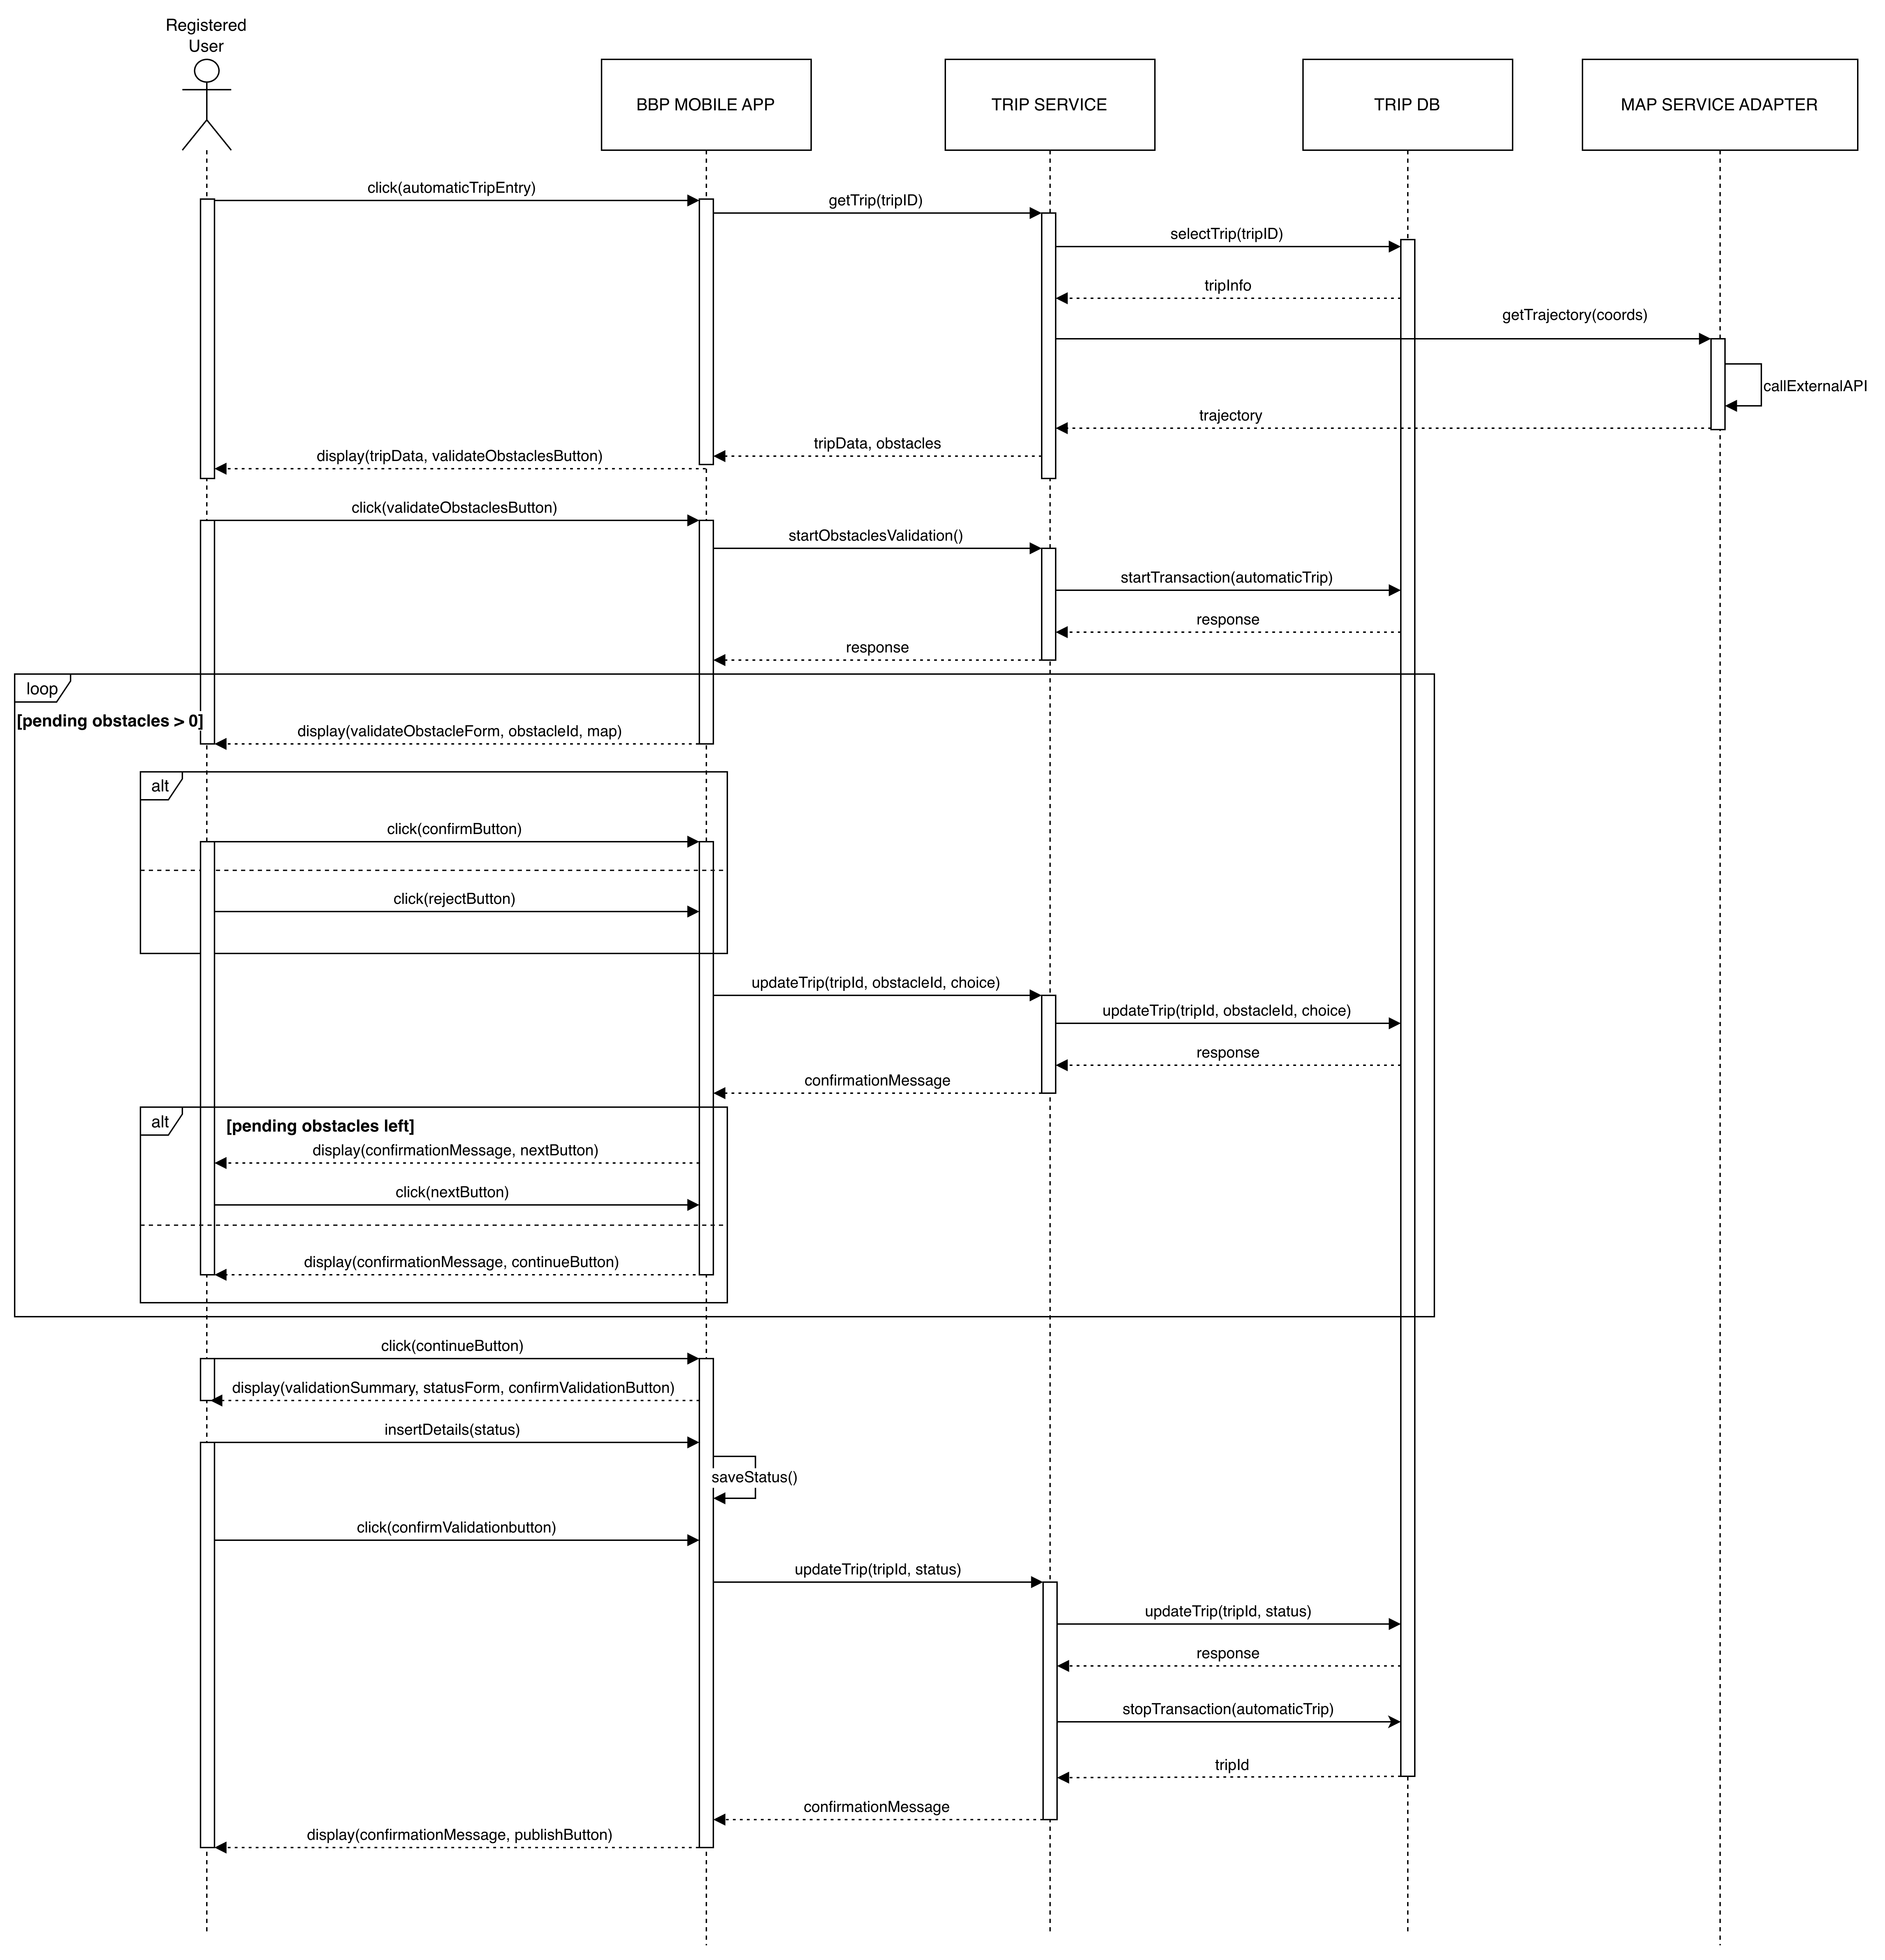
\includegraphics[width=\textwidth]{DD/images/runtime_views/rv5_validate_obstacles.png}
    \caption{Sequence Diagram: Validate Obstacles}
    \label{fig:seq_validate_obstacles}
\end{figure}

% --------------------------------------------------------
% 6. Publish Trip
% --------------------------------------------------------
\subsection{Publish Trip}
The User selects a recorded trip for publication. The Trip Service first validates against the Trip DB that the trip status is "validated" (i.e., no pending obstacles). If eligible, the service anonymizes the data, records the action in the immutable publication log, and produces a \texttt{tripPublished} event to the Message Broker. This ensures the user receives immediate confirmation while the system handles data merging asynchronously.

\begin{figure}[H]
    \centering
    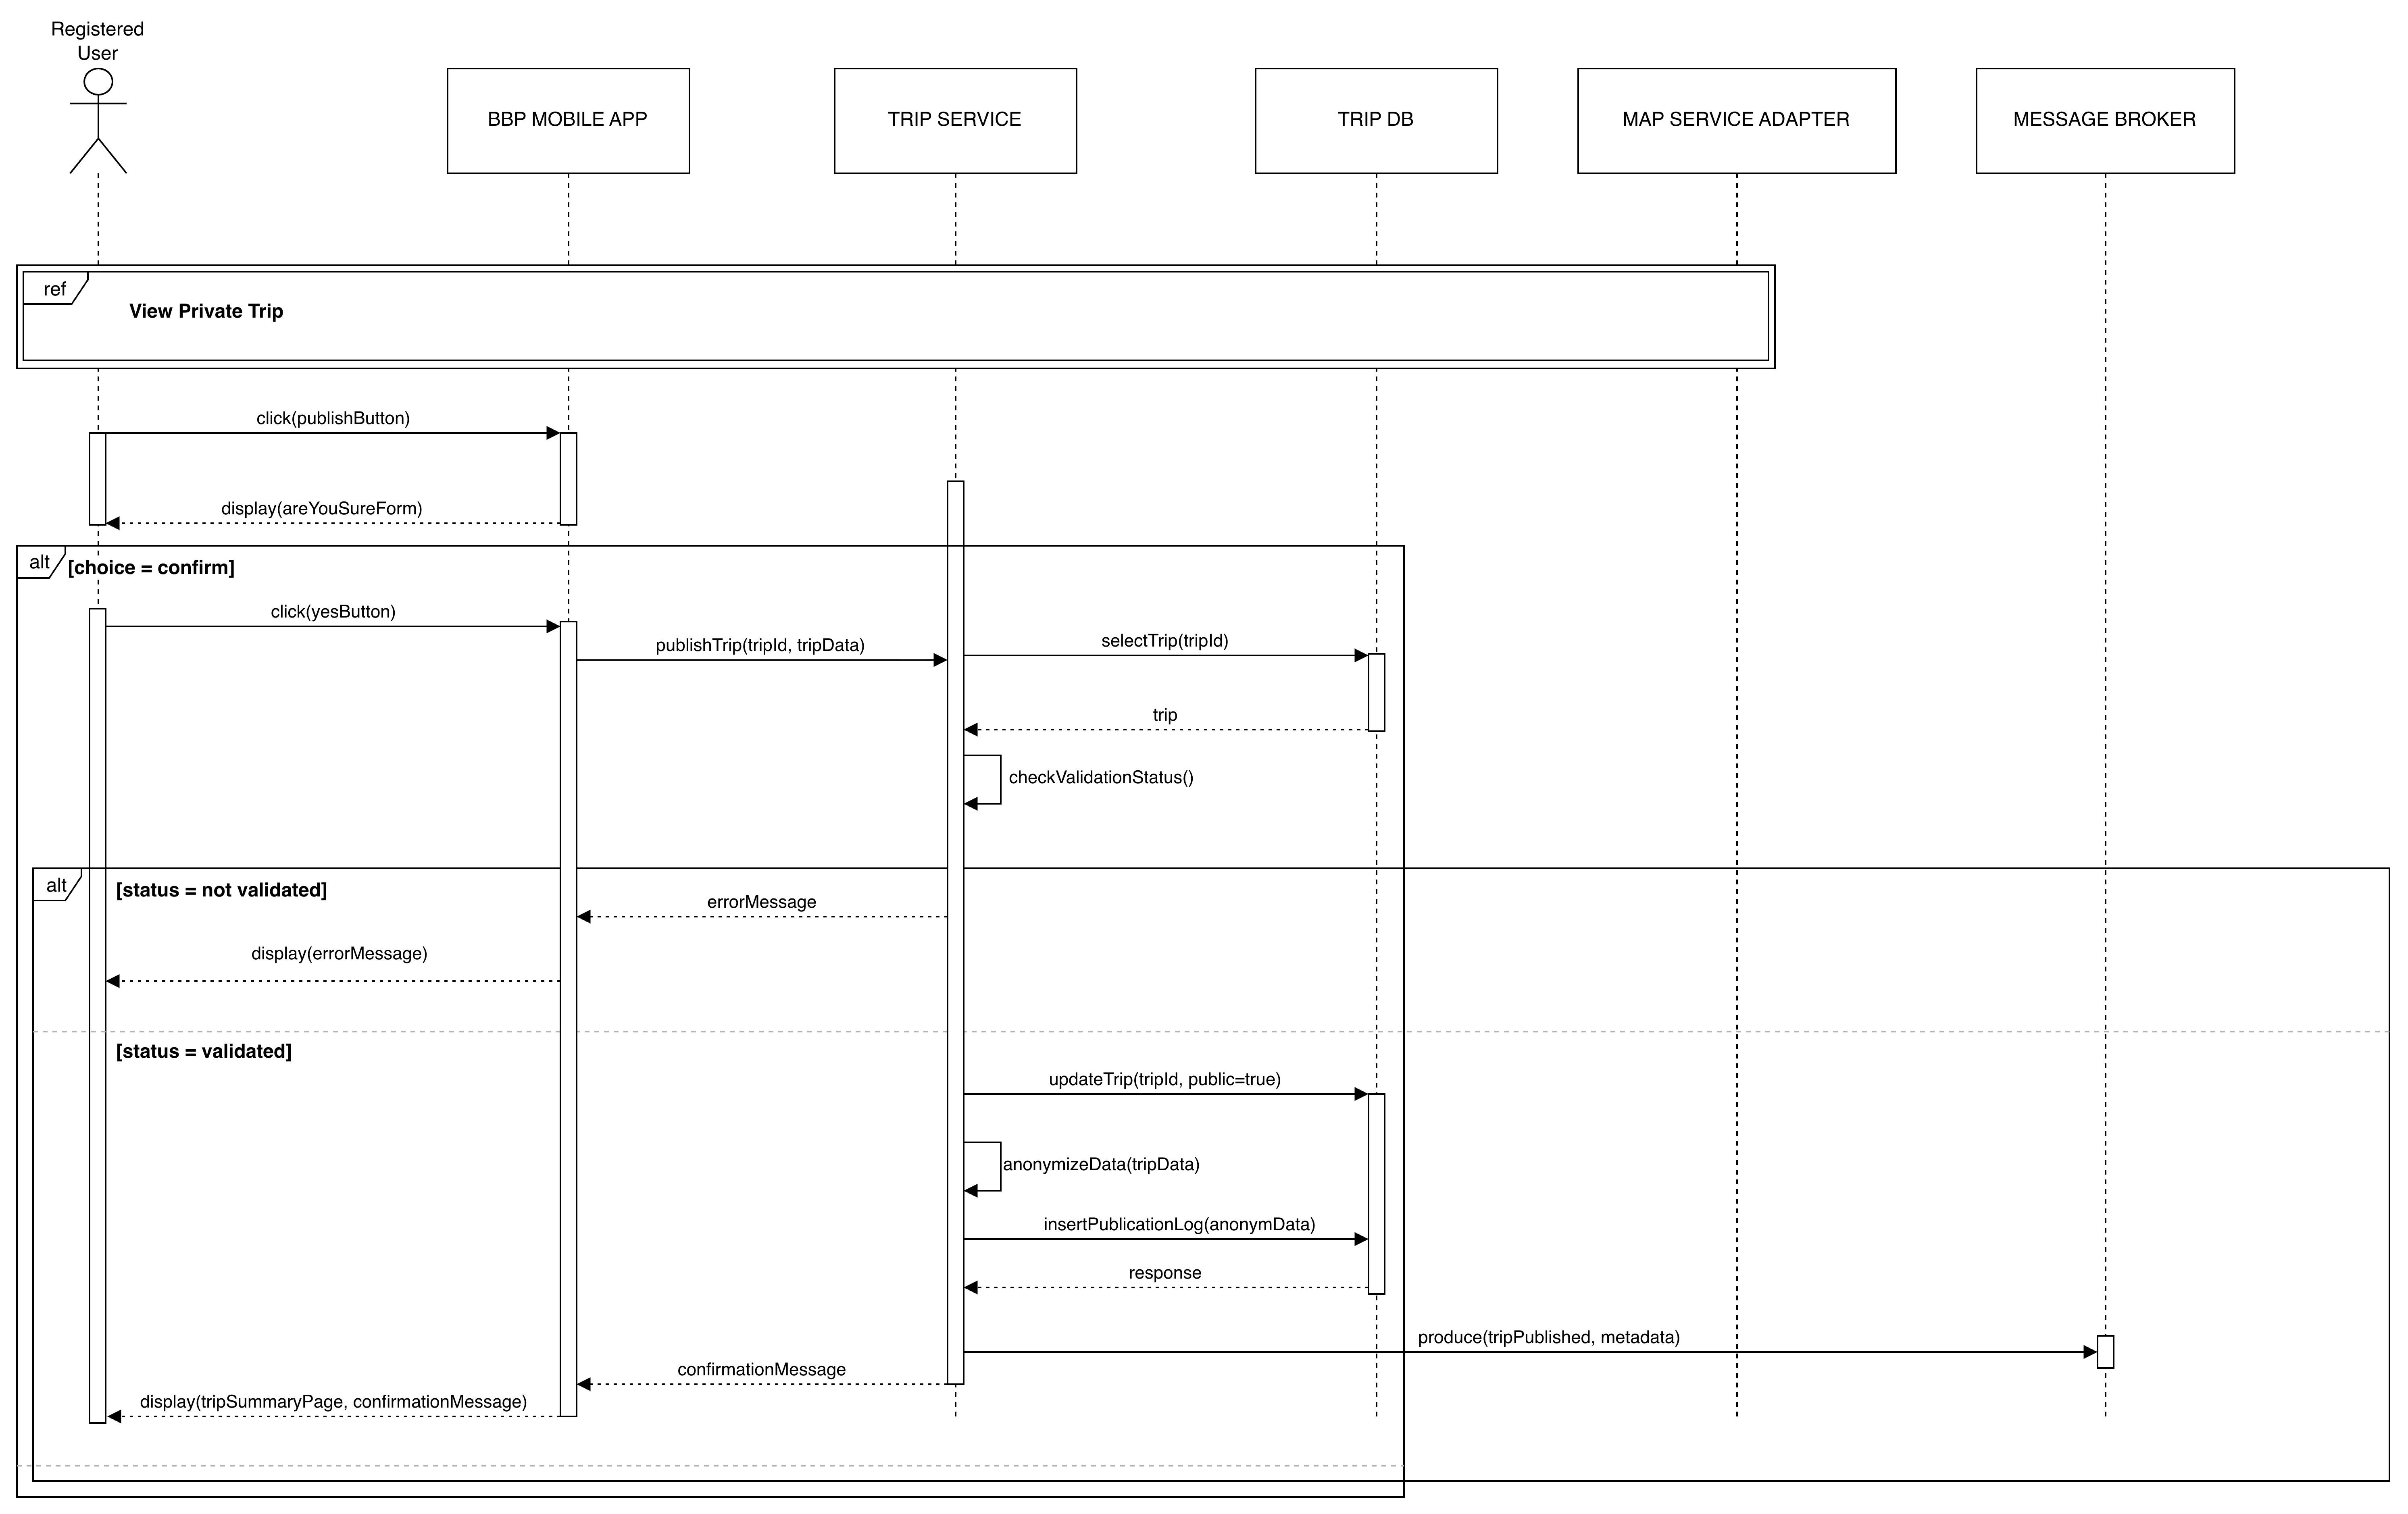
\includegraphics[width=\textwidth]{DD/images/runtime_views/rv6_publish_trip.png}
    \caption{Sequence Diagram: Publish Trip}
    \label{fig:seq_publish_trip}
\end{figure}

% --------------------------------------------------------
% 7. View  Trip
% --------------------------------------------------------
\subsection{View  Trip}
The User requests their travel history. The Trip Service retrieves the list of trips from the Trip DB. Upon selecting a specific entry, the service fetches detailed statistics and invokes the Map Service Adapter to reconstruct the visual route geometry. This interaction with the external provider is safeguarded by the Circuit Breaker pattern. The aggregated data is then returned to the Mobile App for rendering.

\begin{figure}[H]
    \centering
    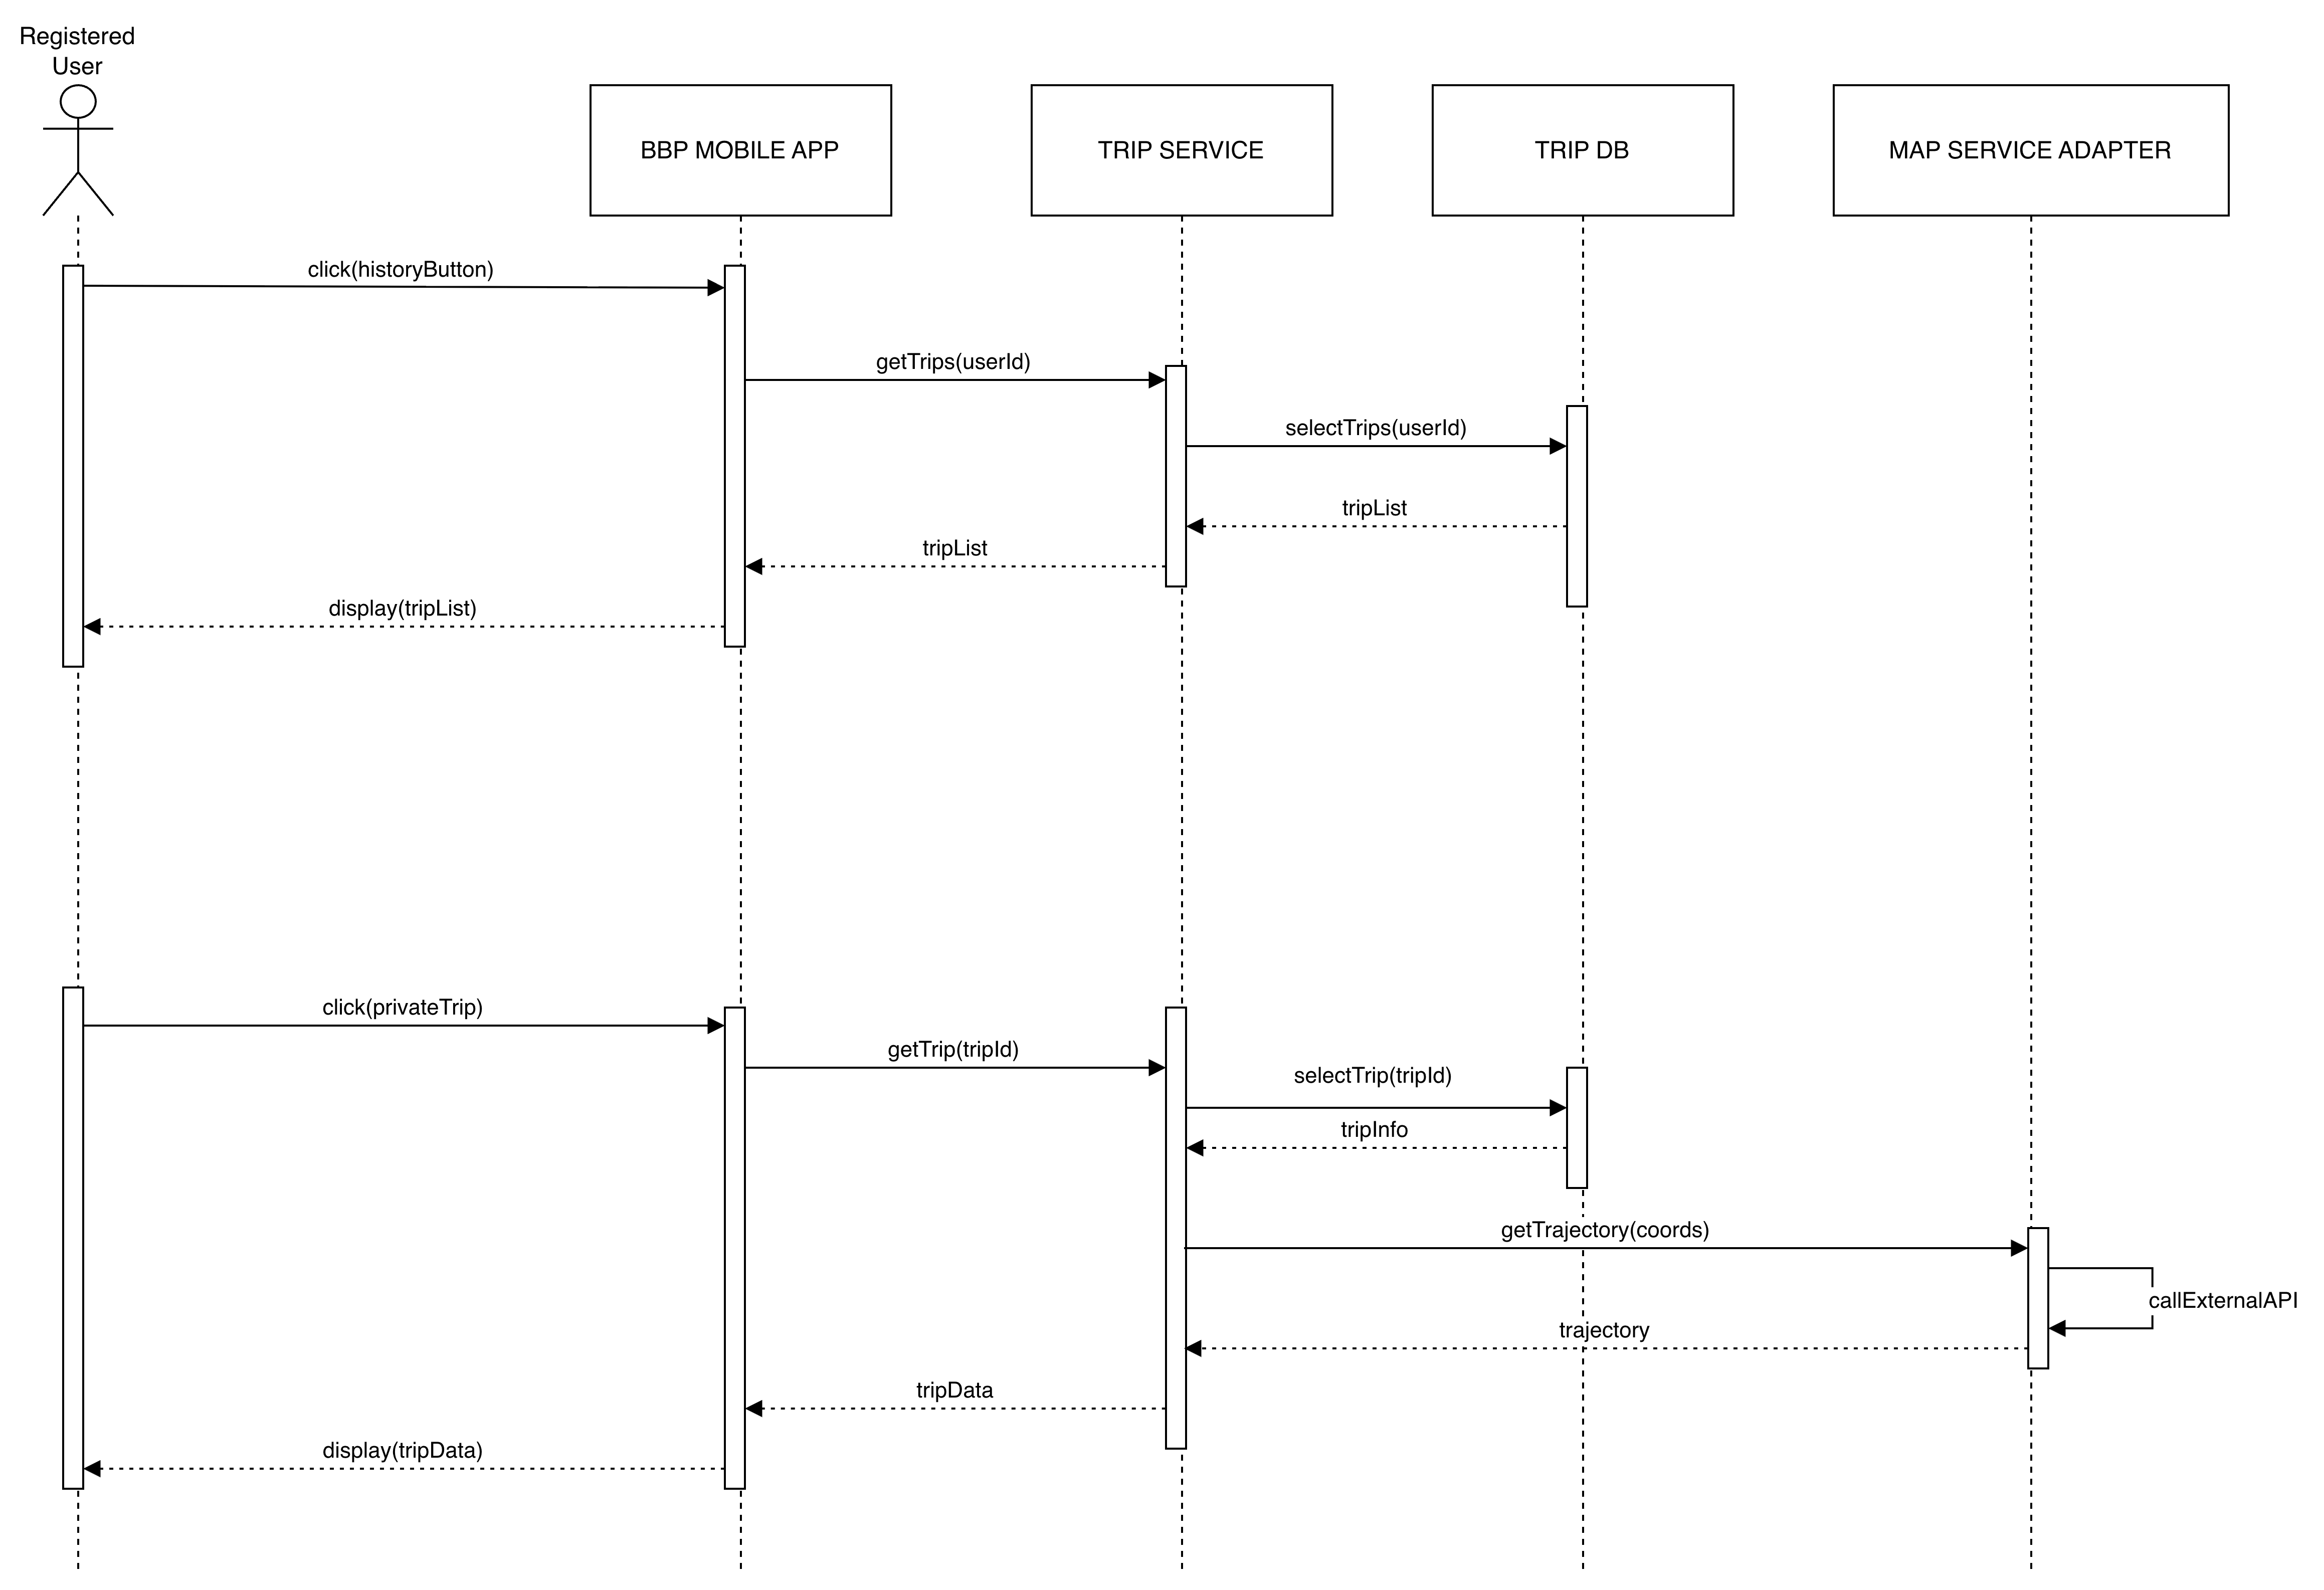
\includegraphics[width=\textwidth]{DD/images/runtime_views/rv7_view_private_trip.png}
    \caption{Sequence Diagram: View Trip}
    \label{fig:seq_view_private_trip}
\end{figure}

% --------------------------------------------------------
% 8. Delete Private Trip
% --------------------------------------------------------
\subsection{Delete Trip}
The User selects a trip from their history and confirms deletion. A synchronous request is sent to the Trip Service, which permanently removes the specific record from the Trip DB. Crucially, this operation is scoped strictly to the private user data; it does not trigger any events to retract data from the public path network, preserving the integrity of previously aggregated community information.

\begin{figure}[H]
    \centering
    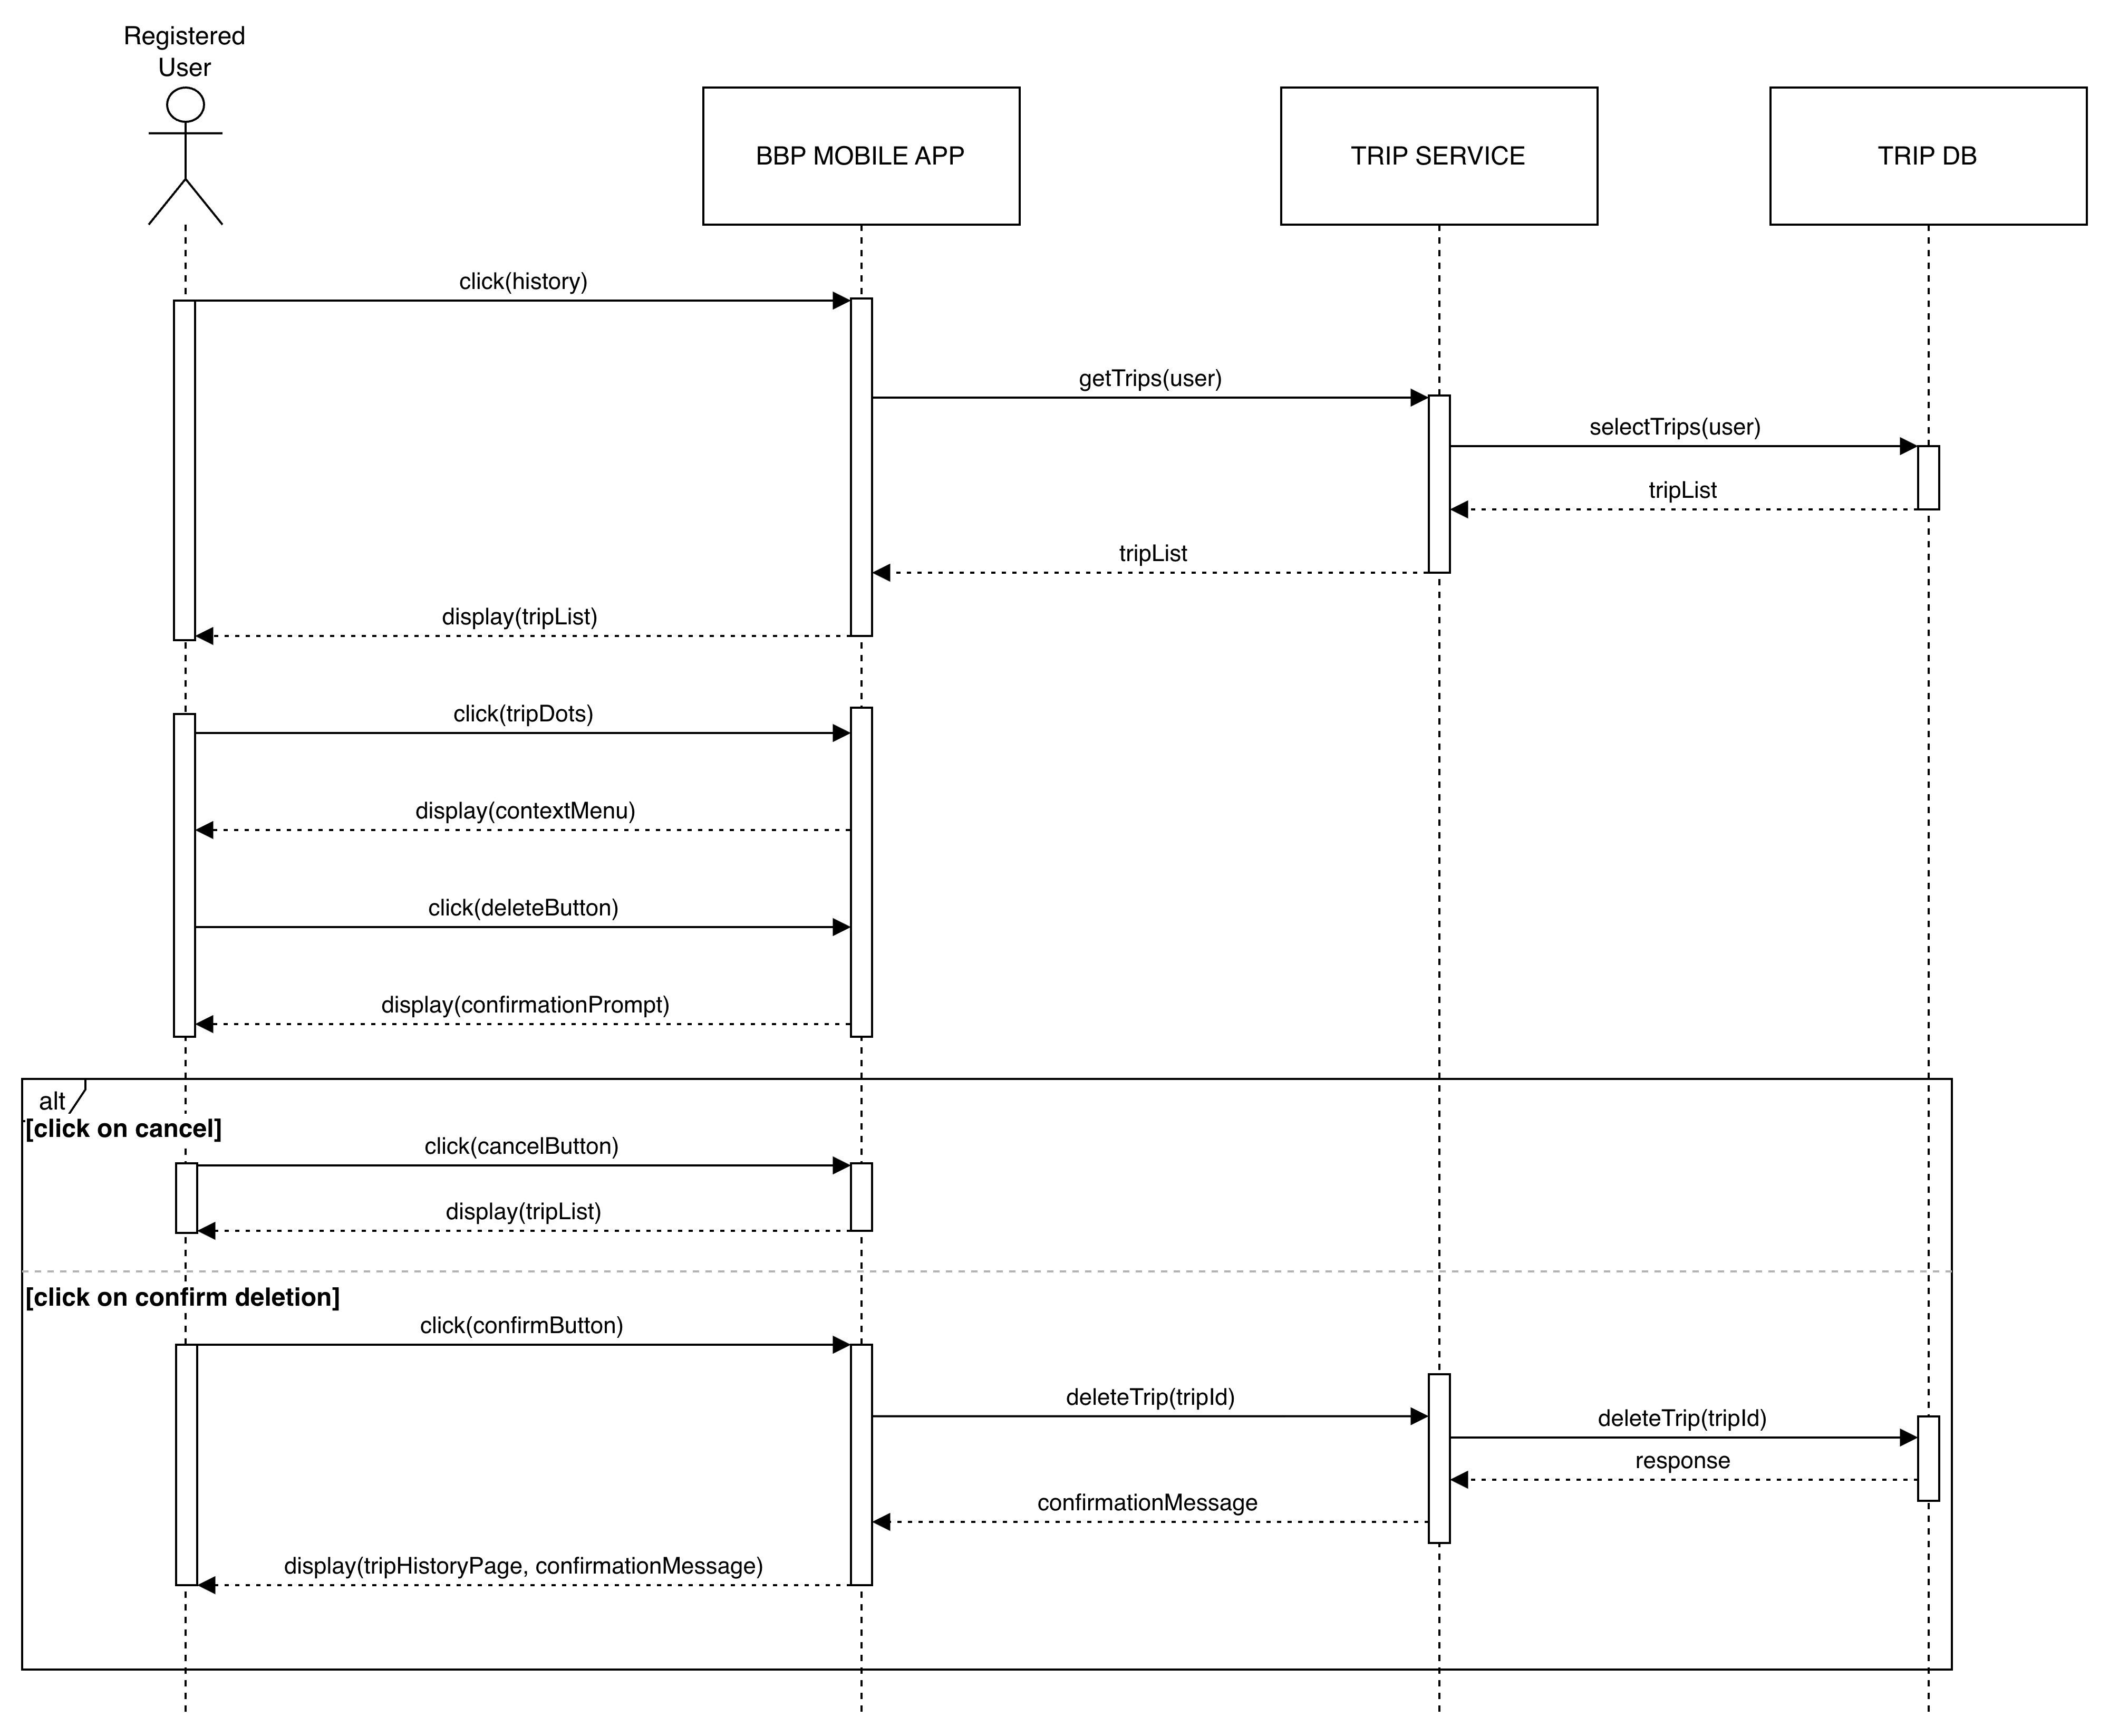
\includegraphics[width=\textwidth]{DD/images/runtime_views/rv8_delete_trip.png}
    \caption{Sequence Diagram: Delete Trip}
    \label{fig:seq_delete_trip}
\end{figure}

% --------------------------------------------------------
% 9. Search Path
% --------------------------------------------------------
\subsection{Search Path}
The User searches for a location via text or map interaction. The Path Service handles the request by invoking the Map Service Adapter to resolve addresses or coordinates (Geocoding/Reverse Geocoding). Once resolved, the service queries the Path DB to retrieve and rank matching routes.

\begin{figure}[H]
    \centering
    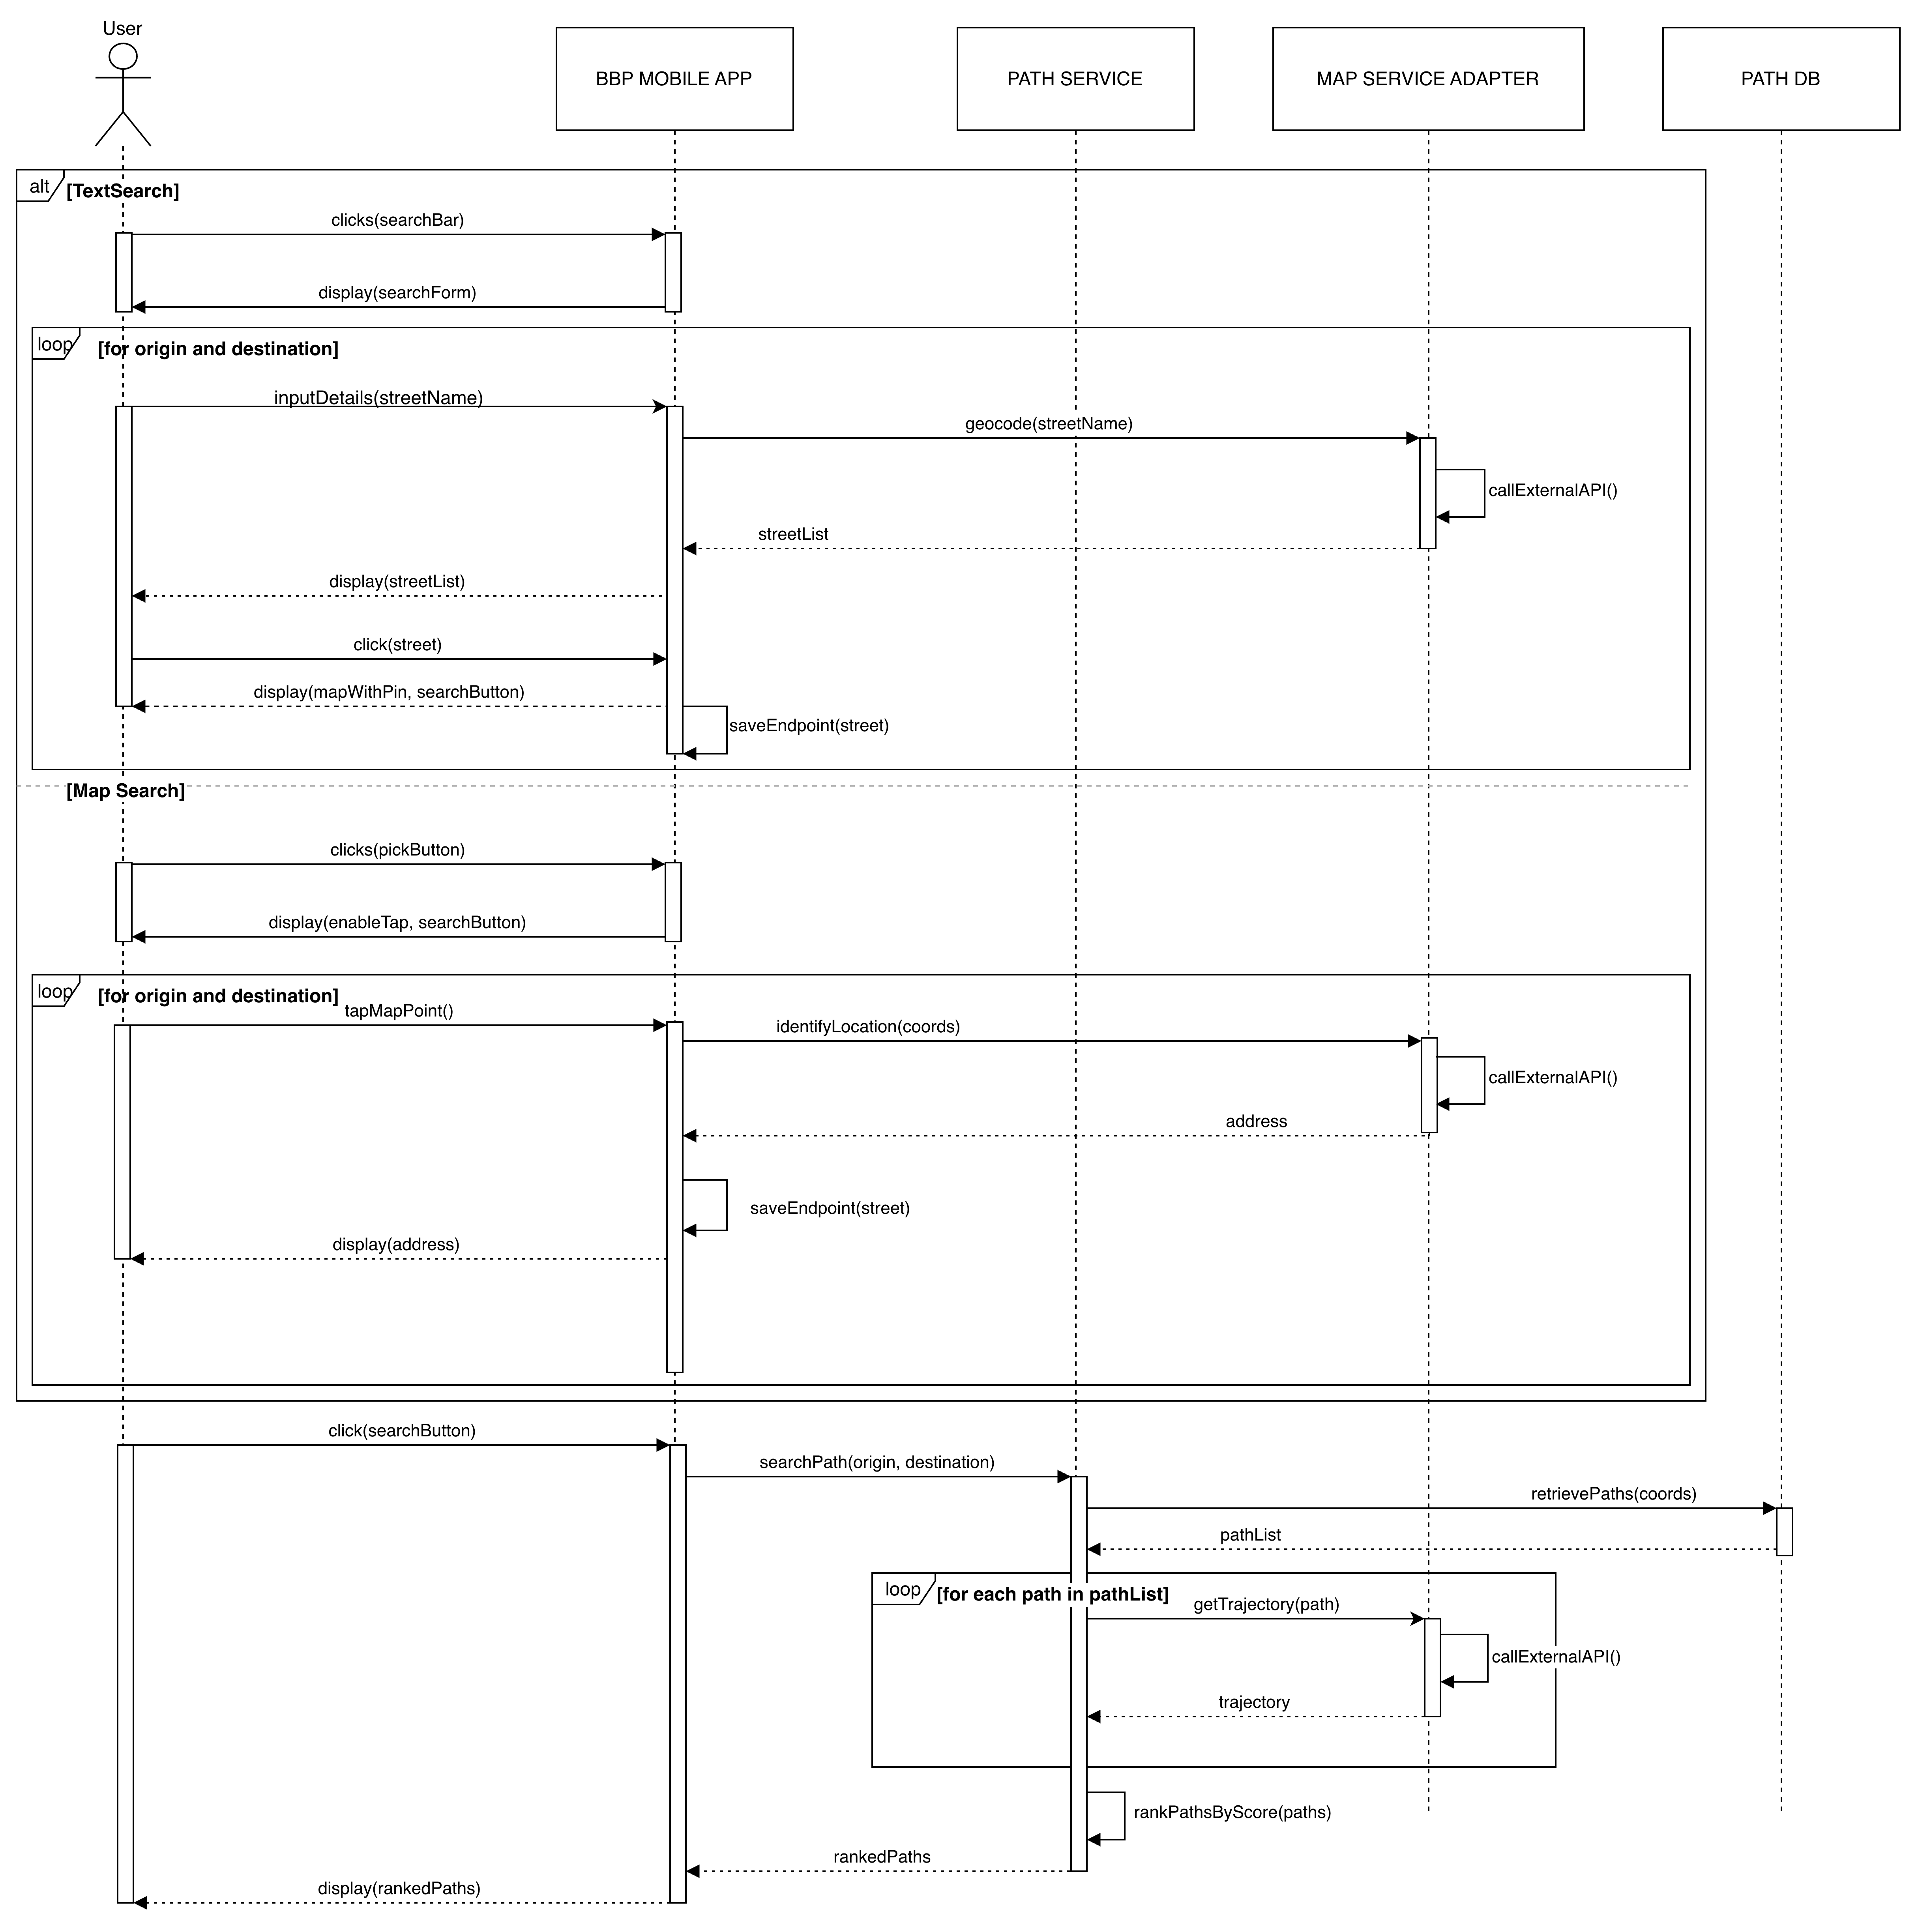
\includegraphics[width=\textwidth]{DD/images/runtime_views/rv9_search_path.png}
    \caption{Sequence Diagram: Search Path}
    \label{fig:seq_search_path}
\end{figure}

% --------------------------------------------------------
% 10. View Path
% --------------------------------------------------------
\subsection{View Path}
The User selects a specific route to view details. The Path Service handles the request by first retrieving the path's metadata from the Path DB. To construct the full visualization, it acts as an aggregator: it fetches the precise trajectory geometry from the Map Service Adapter and the real-time environmental conditions from the Weather Service Adapter. Both synchronous interactions with these external providers are safeguarded by the Circuit Breaker pattern. The service combines these distinct datasets into a unified response, which the Mobile App uses to render the map and path statistics.

\begin{figure}[H]
    \centering
    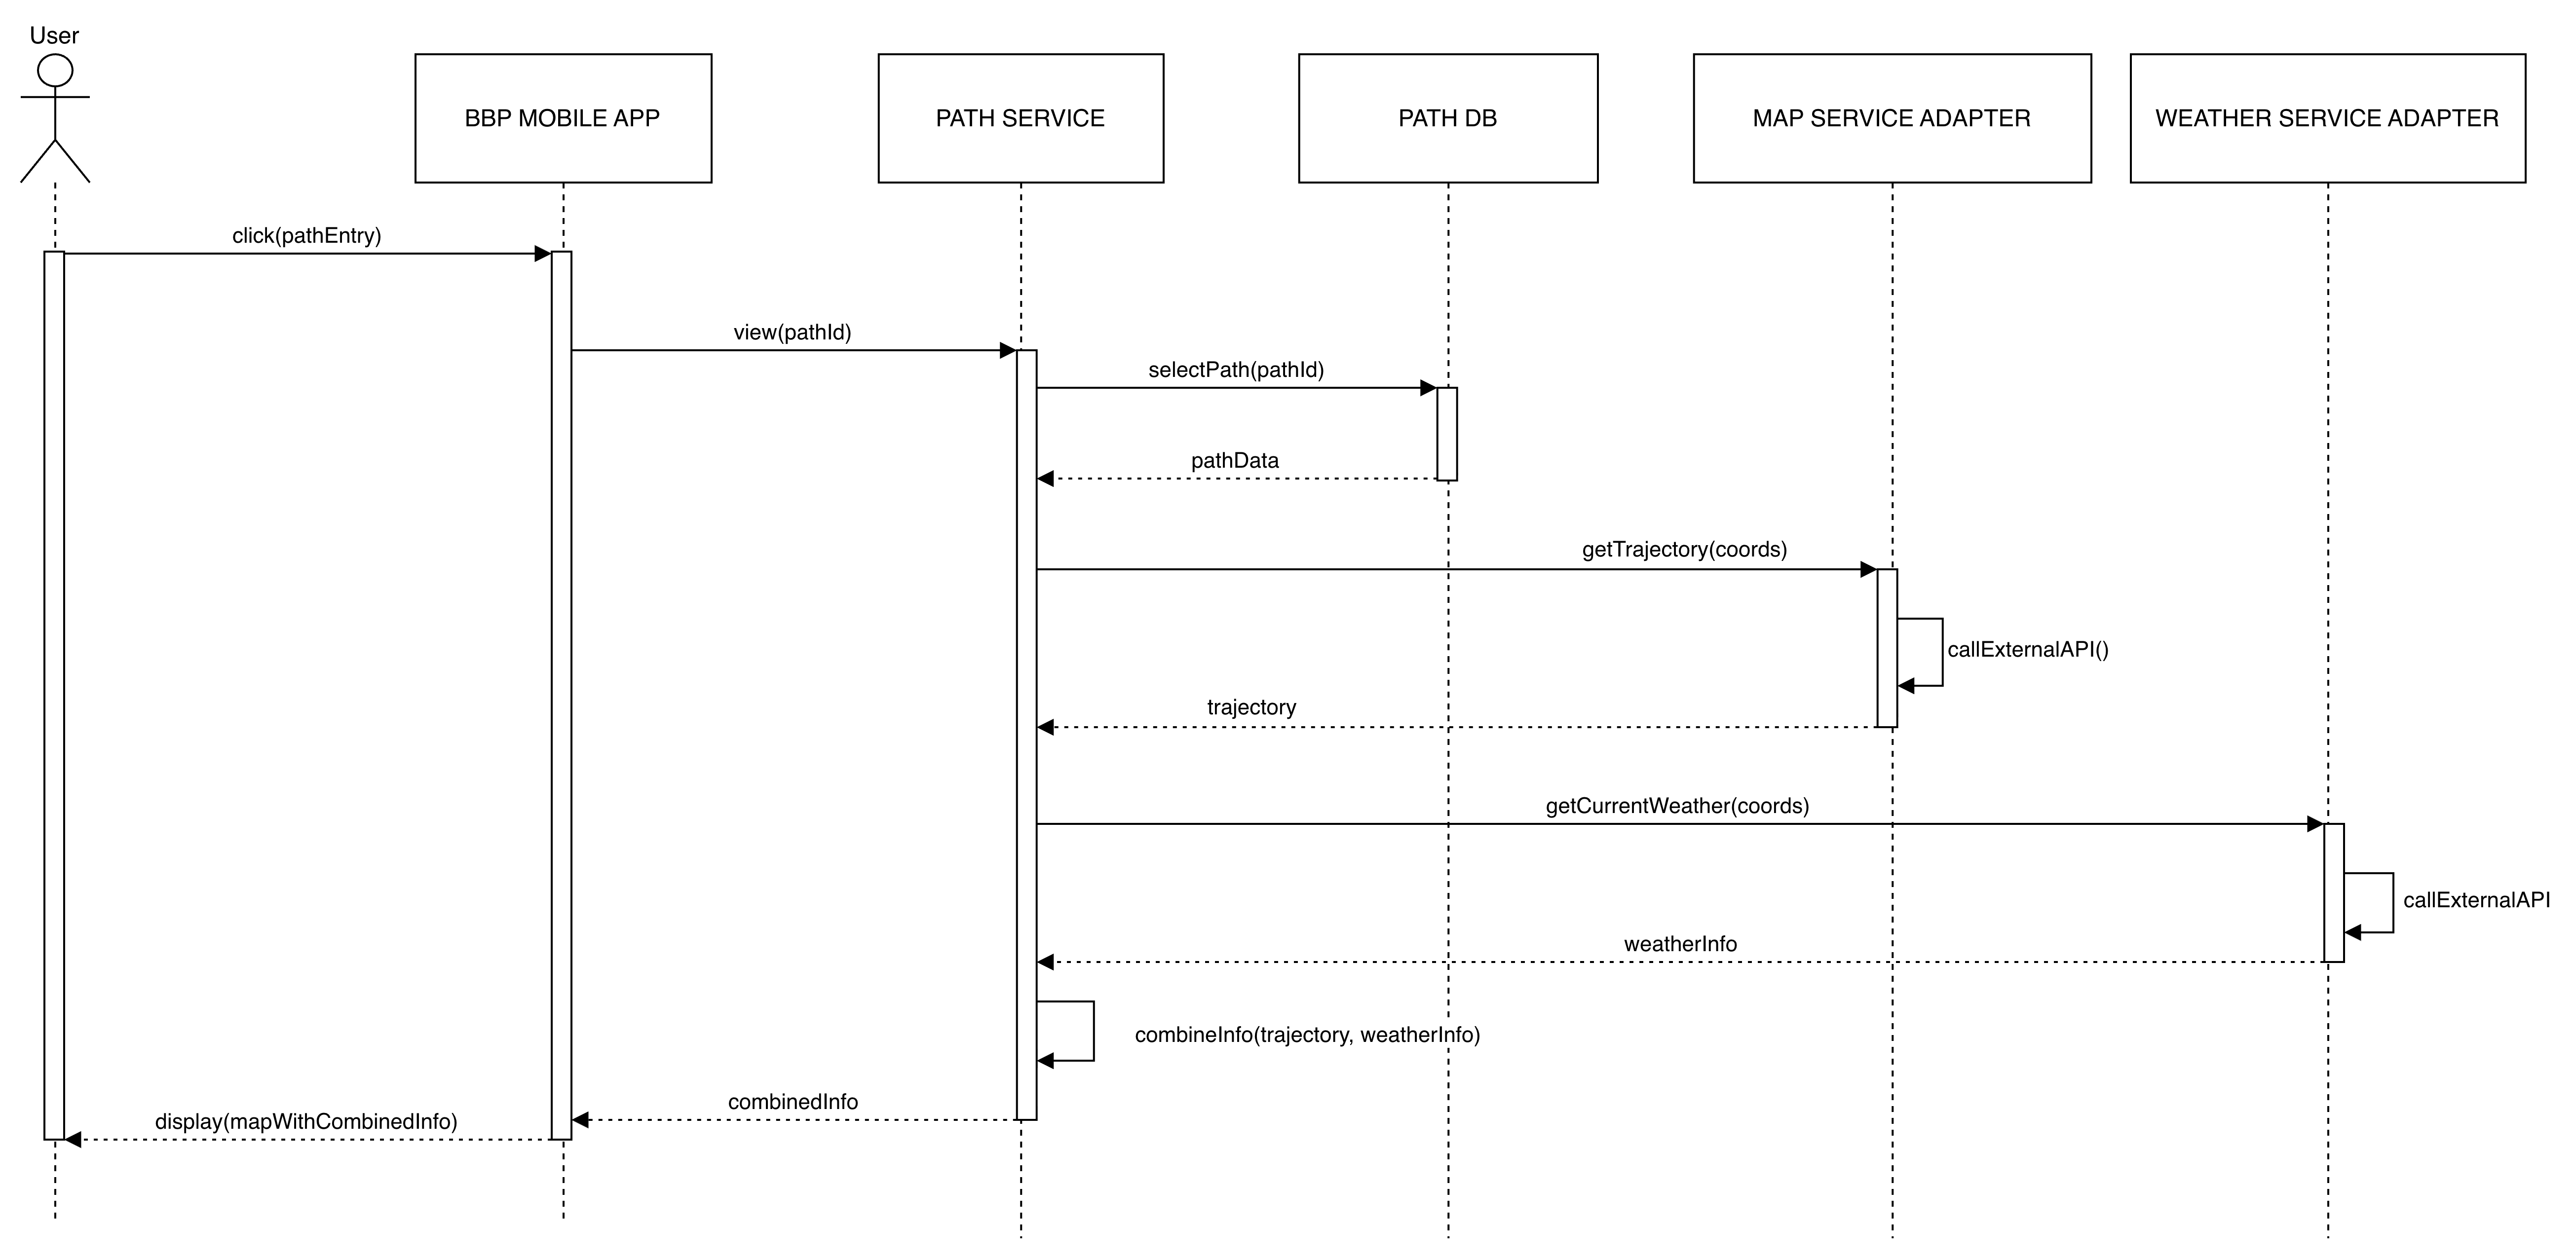
\includegraphics[width=\textwidth]{DD/images/runtime_views/rv10_view_path.png}
    \caption{Sequence Diagram: View Path}
    \label{fig:seq_view_path}
\end{figure}

% --------------------------------------------------------
% 11. Automatic Trip Data Analysis
% --------------------------------------------------------
\subsection{Automatic Trip Data Analysis}
This asynchronous process is triggered when the Message Broker notifies the Analysis Service of a new \texttt{automaticTripRecorded} event. To provide context for the analysis, the service first queries the Weather Service Adapter for historical weather conditions at the time of the trip; this external dependency is protected by the Circuit Breaker pattern. The service then processes the raw sensor data to identify obstacles and calculate performance statistics. Finally, it publishes an \texttt{analysisCompleted} event (containing the detected obstacles), which the Trip Service consumes to update the specific trip record in the Trip DB.

\begin{figure}[H]
    \centering
    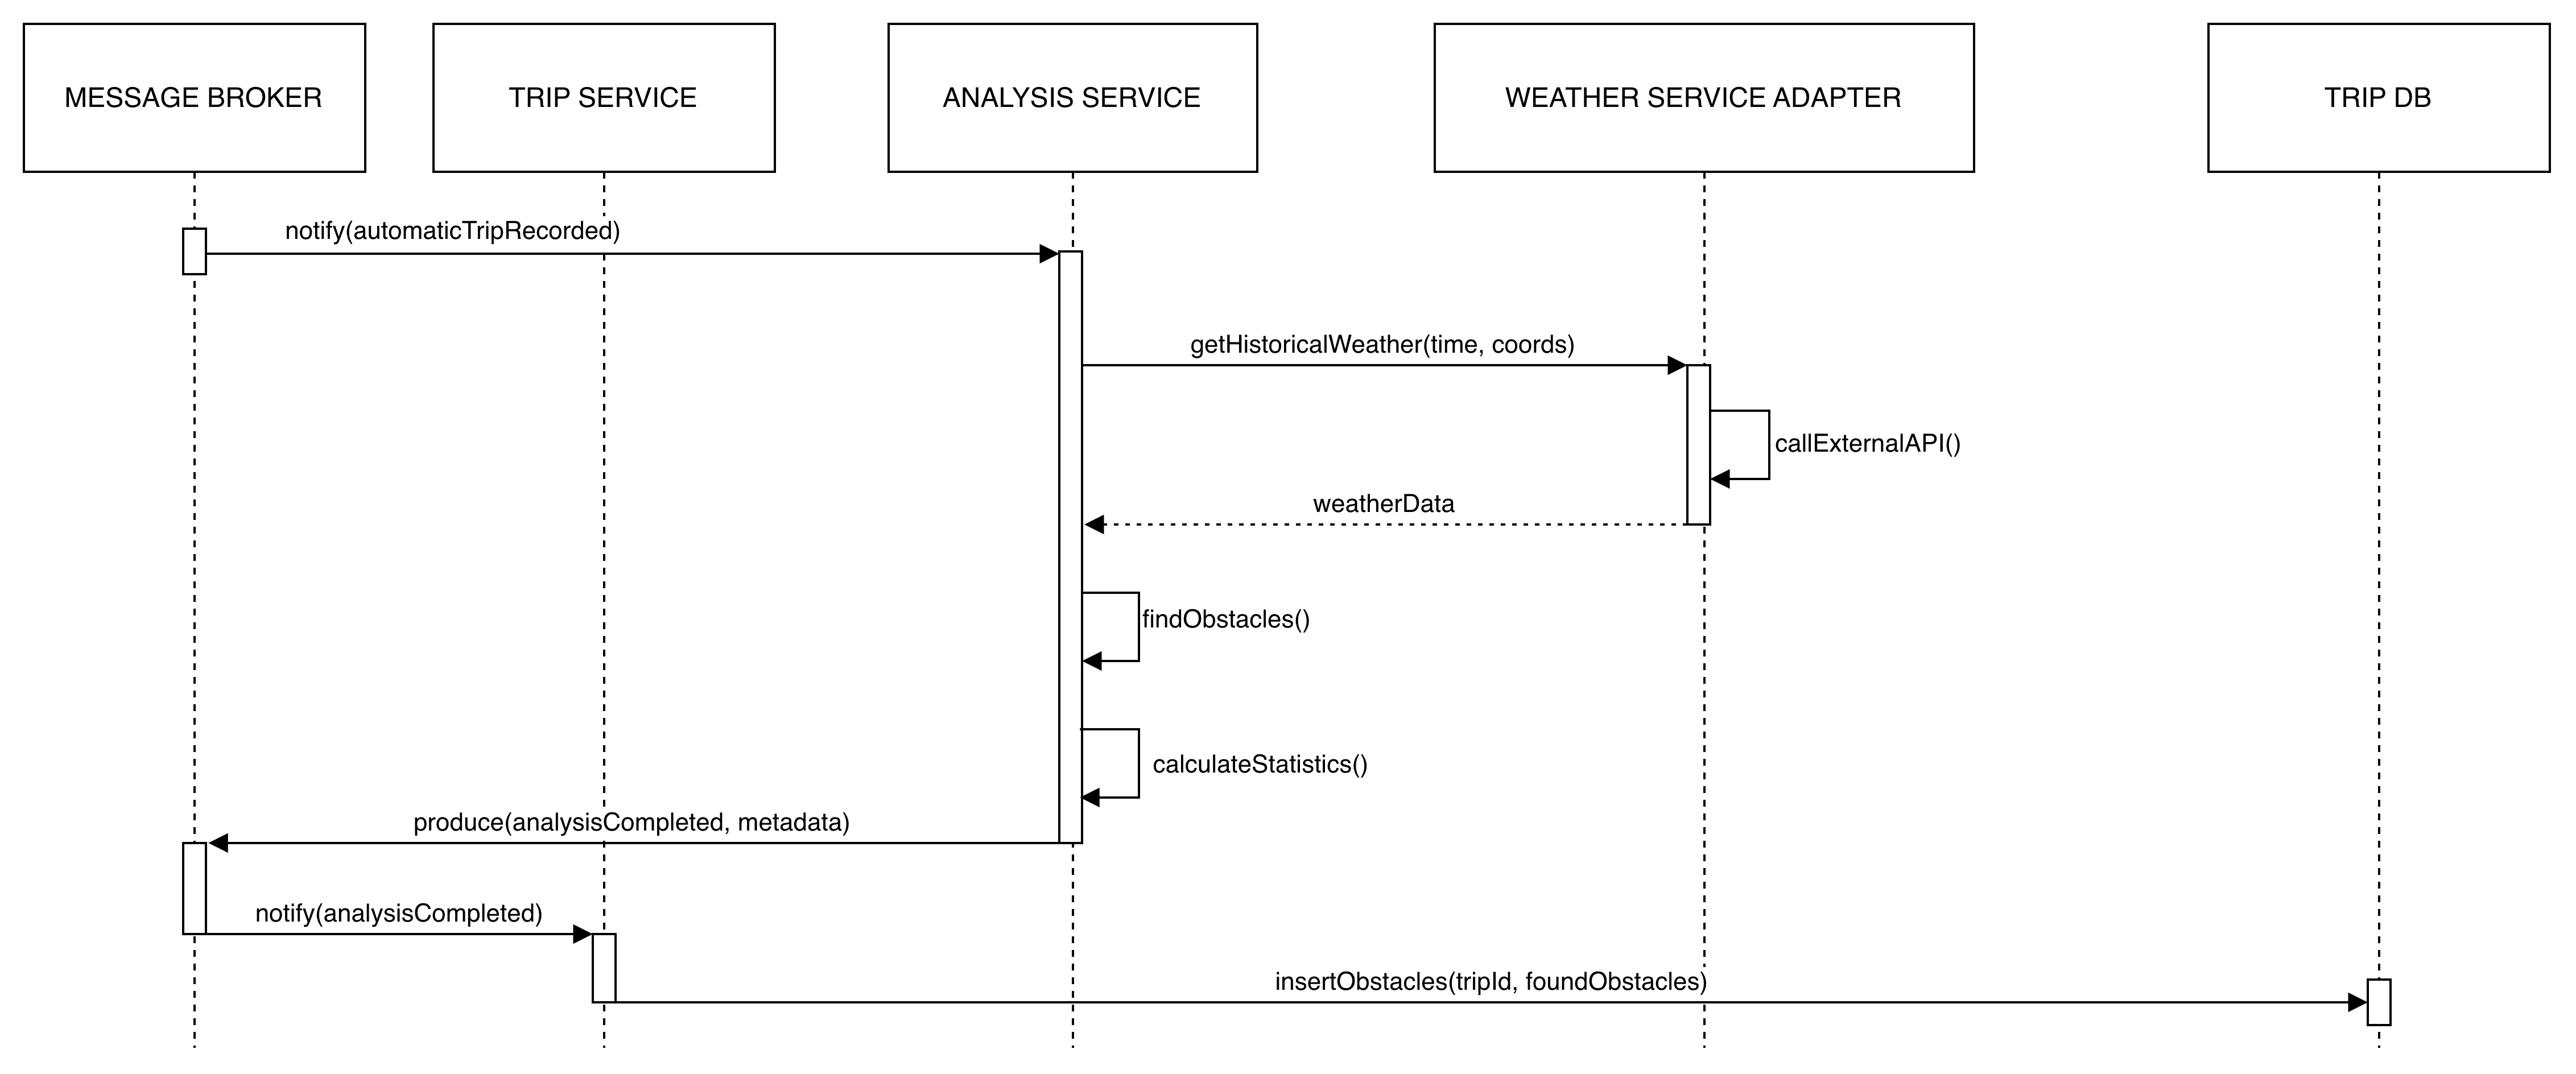
\includegraphics[width=\textwidth]{DD/images/runtime_views/rv11_automatic_trip_data_analysis.png}
    \caption{Sequence Diagram: Automatic Trip Data Analysis}
    \label{fig:seq_trip_analysis}
\end{figure}

% --------------------------------------------------------
% 12. Trip Merging
% --------------------------------------------------------
\subsection{Trip Merging}
This workflow represents the background synchronization between private user contributions and the public path network. It initiates when the Message Broker delivers a \texttt{tripPublished} event to the Merge Service. The service executes aggregation algorithms to merge the new trip data with the existing path, recalculating the global "Path Score" and updating the road status. Upon completion, it publishes a \texttt{mergeCompleted} event. The Path Service consumes this event to update the read-optimized Path DB, ensuring the public search index immediately reflects the latest community data without blocking the user.

\begin{figure}[H]
    \centering
    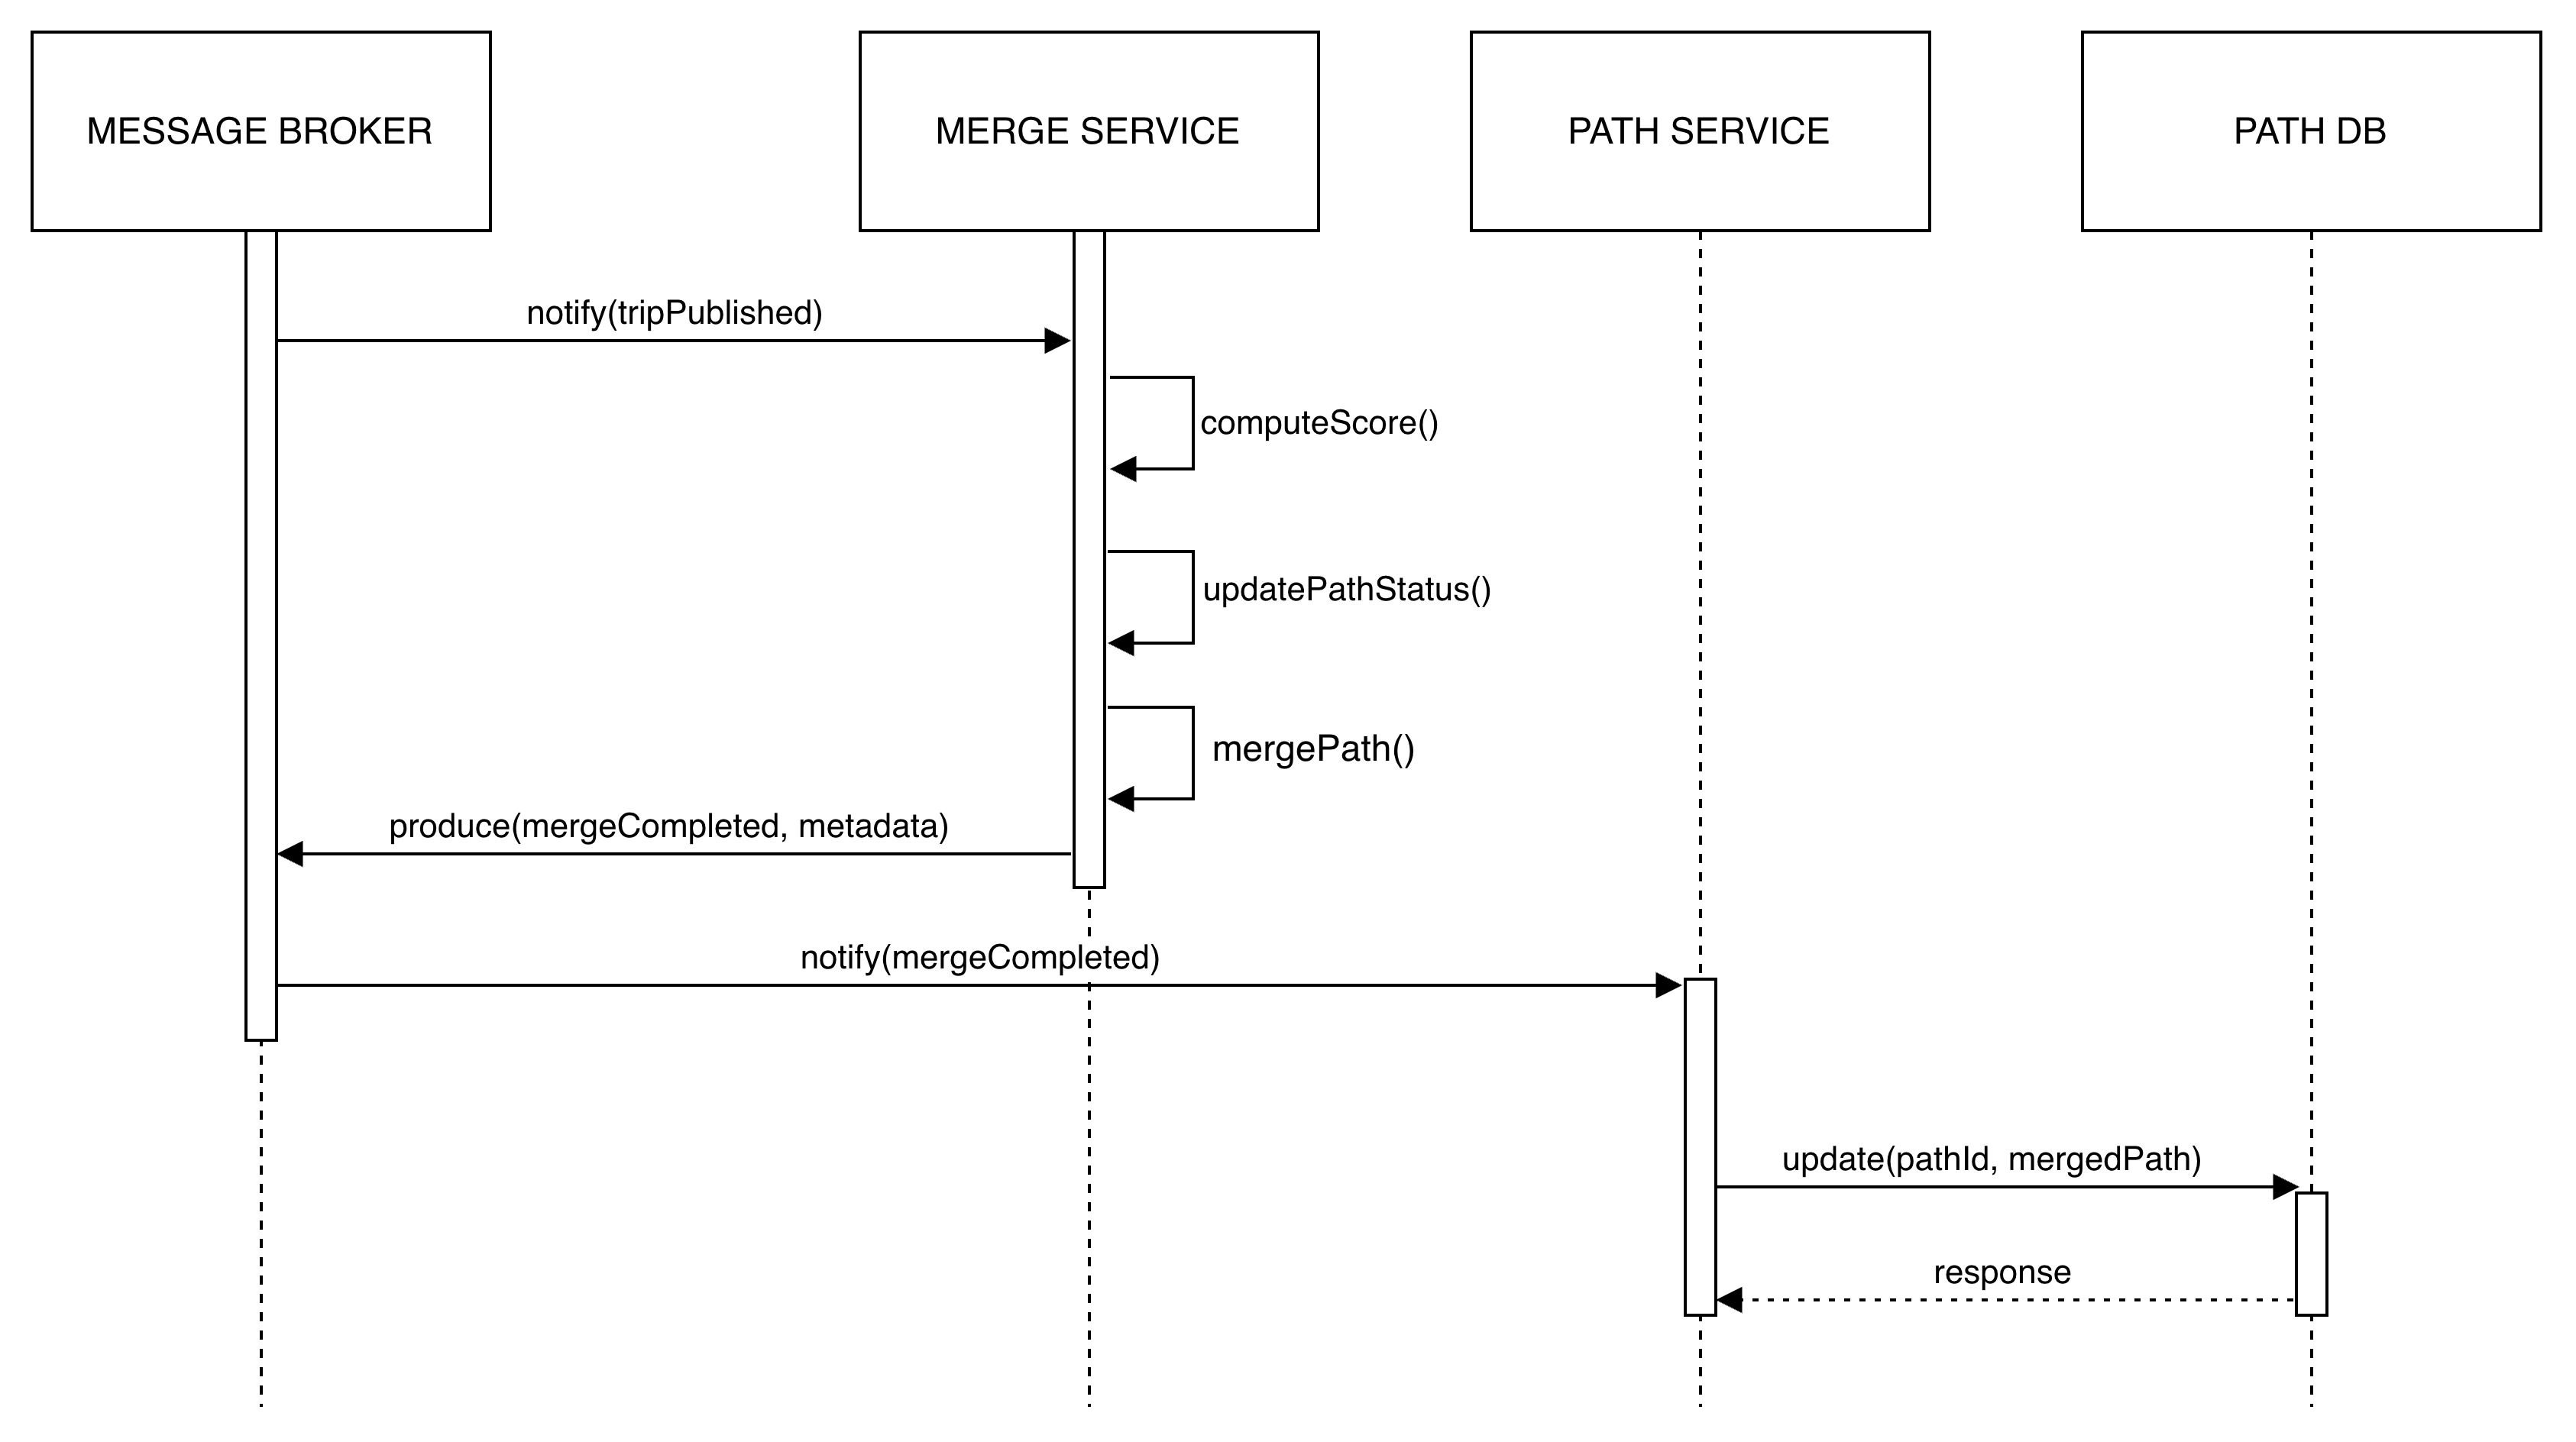
\includegraphics[width=\textwidth]{DD/images/runtime_views/rv12_trip_merging.png}
    \caption{Sequence Diagram: Trip Merging}
    \label{fig:seq_trip_merging}
\end{figure}

% =========================================================
% 2.5 Component Interfaces
% =========================================================
\section{Component Interfaces}

% 2.5.1 Auth Service
\subsection{Auth Service Interface}
Interface offered by the Authentication Service:
\begin{itemize}
    \item \texttt{validateSyntax(email: String, username: String, password: String) : Boolean}
    \item \texttt{hashPassword(password: String) : String}
    \item \texttt{signUp(email: String, username: String, password: String) : Response}
    \item \texttt{logIn(username: String, password: String) : Response}
    \item \texttt{checkCredentials(hashedPassword: String, storedPasswordHash: String) : Boolean}
    \item \texttt{generateSession() : String}
\end{itemize}

% 2.5.2 Trip Service
\subsection{Trip Service Interface}
Interface offered by the Trip Service. It offers all the methods related to Trip, Obstacles and PublicationLog:
\begin{itemize}
    \item \texttt{updateTrip(tripId: int, fieldsToUpdate: Trip) : Response}
    \item \texttt{startRecordingSession()}
    \item \texttt{startManualSession()}
    \item \texttt{syncWithServer(tripId: int, rawData: Object)}
    \item \texttt{saveManualTrip(streets: List<Street>) : Response}
    \item \texttt{addStreet(street: Street, status: PathStatus) : Response}
    \item \texttt{getTrip(tripId: int) : Trip}
    \item \texttt{getTrips(userId: String) : List<Trip>}
    \item \texttt{startObstaclesValidation() : Response}
    \item \texttt{checkValidationStatus() : boolean}
    \item \texttt{publishTrip(tripId: int, tripData: Trip) : Response}
    \item \texttt{anonymizeData(tripData: Trip) : Trip}
    \item \texttt{deleteTrip(tripId: int) : Response}
\end{itemize}

% 2.5.3 Path Service
\subsection{Path Service Interface}
Interface offered by the Path Service:
\begin{itemize}
    \item \texttt{searchPath(origin: GPSCoordinate, destination: GPSCoordinate) : List<Path>}
    \item \texttt{rankPathsByScore(paths: List<Path>) : List<Path>}
    \item \texttt{view(pathId: int) : Path}
    \item \texttt{updatePathStatus() : Response}
    \item \texttt{mergePath() : Path}
    \item \texttt{combineInfo(trajectory: List<GPSCoordinates>, weatherInfo: weather) : Path}
    \item \texttt{computeScore() : double}
\end{itemize}

% 2.5.4 Map Service Adapter
\subsection{Map Service Adapter Interface}
Interface offered by the External Map Service and displayed by the Map Service Adapter:
\begin{itemize}
    \item \texttt{getTrajectory(coords: List<GPSCoordinate>) : List<GPSCoordinate>}
    \item \texttt{geocode(streetName: String) : List<Street>}
    \item \texttt{search(streetName: String) : List<Street>}
    \item \texttt{callExternalAPI() : Object}
    \item \texttt{identifyLocation(coords: GPSCoordinates): String}
\end{itemize}

% 2.5.5 Analysis Service
\subsection{Analysis Service Interface}
\begin{itemize}
    \item \texttt{analyzeTrip(tripId: int) : void}
    \item \texttt{findObstacles(sensors: List<SensorReadings>, trajectory: List<GPSCoordinate>) : List<Obstacle>}
    \item \texttt{calculateStatistics(trip: AutomaticTrip, weather: Weather) : Statistics}
\end{itemize}

% 2.5.6 Weather Service Adapter
\subsection{Weather Service Adapter Interface}
Interface offered by the External Weather Service and displayed by the Weather Service Adapter:
\begin{itemize}
    \item \texttt{getCurrentWeather(coords: GPSCoordinate) : Weather}
    \item \texttt{getHistoricalWeather(time: DateTime, coords: GPSCoordinate) : Weather}
    \item \texttt{callExternalAPI() : Object}
\end{itemize}

% 2.5.7 Auth DB
\subsection{Auth DB Interface}
Interface offered by the AuthDB:
\begin{itemize}
    \item \texttt{insertUser(email: String, username: String, passwordHash: String) : Response}
    \item \texttt{selectUser(username: String) : RegisteredUser}
\end{itemize}

% 2.5.8 Trip DB
\subsection{Trip DB Interface}
Interface offered by the TripDB:
\begin{itemize}
    \item \texttt{startTransaction(tripType: String) : int}
    \item \texttt{stopTransaction(tripType: String) : int}
    \item \texttt{updateTrip(tripId: int, fieldsToUpdate: Trip) : Response}
    \item \texttt{selectTrip(tripId: int) : Trip}
    \item \texttt{insertPublicationLog(anonymData: Trip) : Response}
    \item \texttt{selectTrips(userId: String) : List<Trip>}
    \item \texttt{deleteTrip(tripId: int) : Response}
    \item \texttt{insertObstacles(tripId: int, foundObstacles: List<Obstacle>) : Response}
\end{itemize}

% 2.5.9 Path DB
\subsection{Path DB Interface}
Interface offered by the PathDB:
\begin{itemize}
    \item \texttt{retrievePaths(coords: GPSCoordinate) : List<Path>}
    \item \texttt{selectPath(pathId: int) : Path}
    \item \texttt{update(pathId: int, mergedPath: Path) : Response}
\end{itemize}

% 2.5.10 Message Broker
\subsection{Message Broker Interface}
Interface offered by the Message Broker:
\begin{itemize}
    \item \texttt{produce(event: Event, eventMetadata: Metadata = null) : void}
    \item \texttt{notify(event: Event)}
\end{itemize}

In the sequence diagrams regarding asynchronous workflows (e.g., Data Analysis, Merging), the interaction between the Message Broker and the subscribing services is depicted using the \texttt{notify(Event)} message.

This notation represents the Publish-Subscribe pattern adopted by the architecture. Specifically, it indicates that the microservice is subscribed to a specific Topic. When a new event is published to that topic, the Message Broker pushes a notification to the subscriber. This notification acts as a trigger, automatically invoking the service's internal handling function to consume the event payload and execute the associated business logic.

\paragraph{Event Types:}
\begin{itemize}
    \item \texttt{automaticTripRecorded} - Automatic trip recording completed
    \item \texttt{manualTripCreated} - Manual trip created
    \item \texttt{tripPublished} - Trip made public
    \item \texttt{analysisCompleted} - Trip data analysis finished
    \item \texttt{mergeCompleted} - Trip data merged into paths
\end{itemize}

% =========================================================
% 2.6 Selected Architectural Styles and Patterns
% =========================================================
\section{Selected Architectural Styles and Patterns}

\subsection{Microservices Architecture}
BBP adopts a microservice-based architecture, decomposing the backend into independently deployable services (Authentication, Trip, Path, Analysis, Merge) aligned with distinct business capabilities and data to manage. The role and responsibilities of each microservice are detailed in Section 2.2.2.1.

\subsection{Event-Driven Architecture (EDA)}
The platform follows an event-driven interaction style for background workflows, where services coordinate asynchronously via a Message Broker using publish/subscribe, reducing direct dependencies and improving scalability. The adopted event flows and service subscriptions are described in Section 2.2.2.2.

\subsection{Layered Architecture}
Internally, each microservice is structured according to a layered organization (e.g., interface/controller, business logic, and data access), improving maintainability and testability. This is a standard implementation decision and is consistent with the service responsibilities described in Section 2.2.2.1.

% =========================================================
% 2.7 Other Design Decisions
% =========================================================
\section{Other Design Decisions}

\subsection{API Gateway Pattern}
BBP uses an API Gateway as the single entry point for client interactions, providing a unified access interface and isolating internal services from direct exposure. Its role in request forwarding and separation between client-side and backend logic is introduced in Section 2.2.1 and further reflected in the Deployment View.

\subsection{Circuit Breaker Pattern}
To improve resilience when calling external Map and Weather providers, BBP applies the Circuit Breaker pattern within the corresponding service adapters to prevent cascading failures and fail fast under degraded external conditions. This integration is described in Section 2.2.2.3.

\subsection{Database-per-Service Pattern}
The platform enforces database-per-service ownership, ensuring that each microservice accesses only its own datastore and that cross-service data exchange occurs via APIs or domain events. This constraint is explicitly stated in Section 2.2.3.

\subsection{Databases}
BBP adopts relational databases for AuthDB and PathDB due to the structured nature of authentication and path metadata, while TripDB is implemented as a time-series datastore to efficiently persist high-frequency sensor streams, and includes an append-only PublicationLog to permanently store published trips in an anonymized way. The rationale and data flow are summarized in Section 2.2.3.




